\documentclass[12pt,titlepage]{book}
\usepackage[margin=1in]{geometry} 
\usepackage{amsmath,amsthm,amssymb,graphicx,mathtools,tikz,hyperref}
\usepackage{pgfplots}
\usepackage{xcolor}
\newcommand{\redp}[1]{\textcolor{red}{#1}}
\newcommand{\bluep}[1]{\textcolor{blue}{#1}}
\newcommand{\tealp}[1]{\textcolor{teal}{#1}}
\usepackage{tcolorbox}
\newtcolorbox{mybox}{colback=red!5!white,colframe=red!75!black,fonttitle=\bfseries,title=Question}
\newtcolorbox{mybox2}{colback=blue!5!white,colframe=blue!75!black,fonttitle=\bfseries,title=Answer}
\newtcolorbox{qt}{colback=orange!5!white,colframe=orange!75!white}
\usetikzlibrary{patterns,hobby}
\numberwithin{equation}{section}
\usepackage{wrapfig}
\usepackage{indentfirst}
\usepackage{ragged2e}
\RaggedRightParindent = 24 pt
\setlength{\parskip}{0.8em}
\renewcommand{\baselinestretch}{1.5}
\usepackage[noline]{algorithm2e}
\SetAlFnt{\footnotesize}
\usepackage{graphicx}
\usepackage{titling}
\renewcommand\maketitlehooka{\null\mbox{}\vfill}
\renewcommand\maketitlehookd{\vfill\null}
\usepackage{tocloft}
\renewcommand\cftsecafterpnum{\vskip6pt}
\usepackage{makeidx}
\makeindex
\usepackage{mdframed}
\newenvironment{que}
    { \begin{mdframed}[backgroundcolor=green!20] \textbf{$\Delta$ Question} \\}
    {  \end{mdframed}}
\newenvironment{thm}
    { \begin{mdframed}[backgroundcolor=orange!20] \textbf{$\Delta$ Theorem} \\}
    {  \end{mdframed}}
\newenvironment{defi}
    { \begin{mdframed}[backgroundcolor=red!10] \textbf{$\Delta$ Definition} \\}
    {  \end{mdframed}}
\newenvironment{lemma}
    { \begin{mdframed}[backgroundcolor=gray!10] \textbf{$\cdot$ Lemma} \\}
    {  \end{mdframed}}
\newenvironment{example}
    { \begin{mdframed}[backgroundcolor=white!10] \textbf{$\cdot$ Example} \\}
    {  \end{mdframed}}
\usepackage{graphicx}
\usepackage{float}
\usepackage{longtable}
\usepackage{tikz}
\usepackage{esint}
\usepackage{CJKutf8}

\title{Things before QFT for Sloppy Engineers}
\author{Sizhe Liu\\University of Illinois at Urbana-Champaign }
\date{Version 1.0}

\pgfplotsset{compat=1.15}
\begin{document}

\maketitle
\tableofcontents
\chapter{Classic Mechanics}
\section{Formulations}
we call the description of a given theory in a particular mathematical arena a formulation of the theory.

\textbf{Lagrangian}
$$
L=T-V
$$
where $T$ denotes the kinetic energy and $V$ the potential energy.

\textbf{Euler-Lagrange equation}
$$
\frac{\partial L}{\partial q}-\frac{d}{d t}\left(\frac{\partial L}{\partial \dot{q}}\right)=0
$$

\textbf{Hamiltonian}
$$
H=p \dot{q}-L
$$
where $p$ denotes the momentum, $\dot{q}$ the velocity and $L,$ as before,
the Lagrangian. 

\textbf{Hamiltonian's equation}
$$
\begin{array}{l}{\frac{d p}{d t}=-\frac{\partial H}{\partial q}} \\ {\frac{d q}{d t}=\frac{\partial H}{\partial p}}\end{array}
$$

\begin{qt}
\begin{center}
    \tikzset{every picture/.style={line width=0.75pt}} %set default line width to 0.75pt
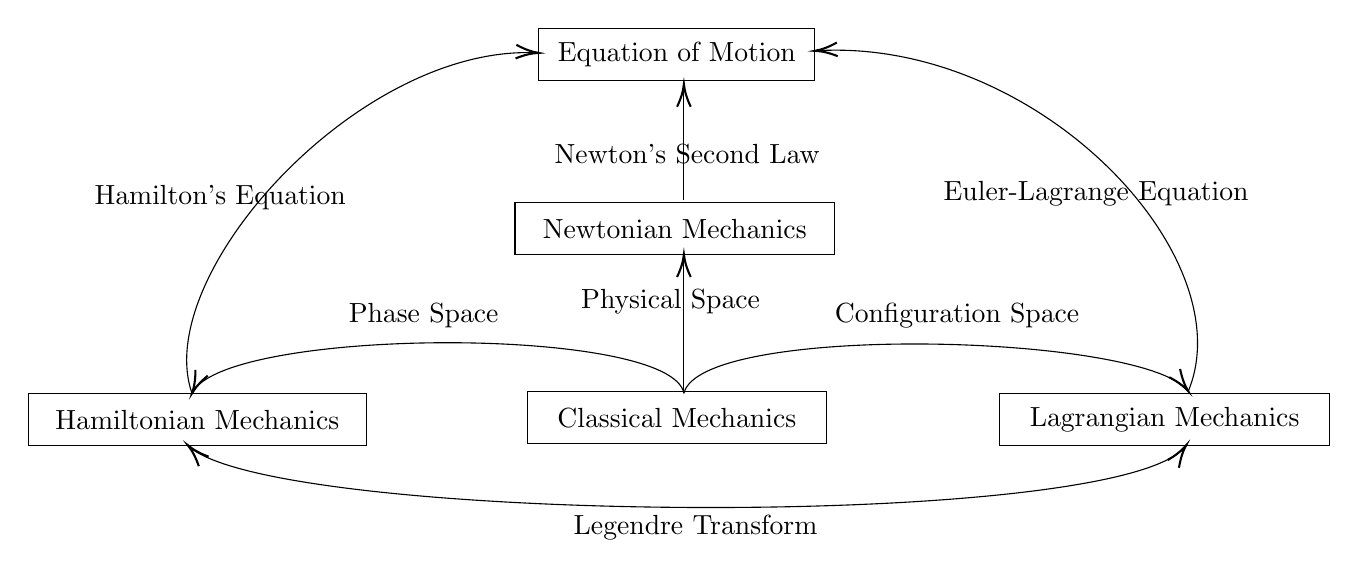
\begin{tikzpicture}[x=0.75pt,y=0.75pt,yscale=-1,xscale=1]
%uncomment if require: \path (0,300); %set diagram left start at 0, and has height of 300

%Straight Lines [id:da6596978253438757] 
\draw    (319.4,108.4) -- (319.4,54.4) ;
\draw [shift={(319.4,52.4)}, rotate = 450] [color={rgb, 255:red, 0; green, 0; blue, 0 }  ][line width=0.75]    (10.93,-3.29) .. controls (6.95,-1.4) and (3.31,-0.3) .. (0,0) .. controls (3.31,0.3) and (6.95,1.4) .. (10.93,3.29)   ;

%Straight Lines [id:da9635704269170282] 
\draw    (319.4,201.4) -- (319.4,136.4) ;
\draw [shift={(319.4,134.4)}, rotate = 450] [color={rgb, 255:red, 0; green, 0; blue, 0 }  ][line width=0.75]    (10.93,-3.29) .. controls (6.95,-1.4) and (3.31,-0.3) .. (0,0) .. controls (3.31,0.3) and (6.95,1.4) .. (10.93,3.29)   ;

%Curve Lines [id:da8601213705090224] 
\draw    (319.4,201.4) .. controls (313.49,168.89) and (103.83,169.38) .. (83.21,199.98) ;
\draw [shift={(82.4,201.4)}, rotate = 295.11] [color={rgb, 255:red, 0; green, 0; blue, 0 }  ][line width=0.75]    (10.93,-3.29) .. controls (6.95,-1.4) and (3.31,-0.3) .. (0,0) .. controls (3.31,0.3) and (6.95,1.4) .. (10.93,3.29)   ;

%Curve Lines [id:da5496082538732877] 
\draw    (319.4,201.4) .. controls (327.28,167.91) and (535.03,172.26) .. (561.33,199.16) ;
\draw [shift={(562.4,200.4)}, rotate = 233.13] [color={rgb, 255:red, 0; green, 0; blue, 0 }  ][line width=0.75]    (10.93,-3.29) .. controls (6.95,-1.4) and (3.31,-0.3) .. (0,0) .. controls (3.31,0.3) and (6.95,1.4) .. (10.93,3.29)   ;

%Curve Lines [id:da6432080478617446] 
\draw    (82.33,228.09) .. controls (129.49,264.15) and (525.01,267.7) .. (560.44,227.63) ;
\draw [shift={(561.4,226.4)}, rotate = 484.44] [color={rgb, 255:red, 0; green, 0; blue, 0 }  ][line width=0.75]    (10.93,-3.29) .. controls (6.95,-1.4) and (3.31,-0.3) .. (0,0) .. controls (3.31,0.3) and (6.95,1.4) .. (10.93,3.29)   ;
\draw [shift={(80.4,226.4)}, rotate = 45.61] [color={rgb, 255:red, 0; green, 0; blue, 0 }  ][line width=0.75]    (10.93,-3.29) .. controls (6.95,-1.4) and (3.31,-0.3) .. (0,0) .. controls (3.31,0.3) and (6.95,1.4) .. (10.93,3.29)   ;
%Curve Lines [id:da7865585332239224] 
\draw    (82.4,201.4) .. controls (62.5,144.68) and (162.39,33.52) .. (248.11,37.33) ;
\draw [shift={(249.4,37.4)}, rotate = 183.33] [color={rgb, 255:red, 0; green, 0; blue, 0 }  ][line width=0.75]    (10.93,-3.29) .. controls (6.95,-1.4) and (3.31,-0.3) .. (0,0) .. controls (3.31,0.3) and (6.95,1.4) .. (10.93,3.29)   ;

%Curve Lines [id:da532295931617982] 
\draw    (562.4,200.4) .. controls (589.26,135.72) and (490.4,30.46) .. (384,36.3) ;
\draw [shift={(382.4,36.4)}, rotate = 356.26] [color={rgb, 255:red, 0; green, 0; blue, 0 }  ][line width=0.75]    (10.93,-3.29) .. controls (6.95,-1.4) and (3.31,-0.3) .. (0,0) .. controls (3.31,0.3) and (6.95,1.4) .. (10.93,3.29)   ;



% Text Node
\draw (325,266) node   [align=left] {Legendre Transform};
% Text Node
\draw (194,164) node   [align=left] {Phase Space};
% Text Node
\draw (451,164) node   [align=left] {Configuration Space};
% Text Node
\draw (313,157) node   [align=left] {Physical Space};
% Text Node
\draw (96,107) node   [align=left] {Hamilton's Equation};
% Text Node
\draw (518,105) node   [align=left] {Euler-Lagrange Equation};
% Text Node
\draw (321,86) node   [align=left] {Newton's Second Law};
% Text Node
\draw    (3.5,201.5) -- (166.5,201.5) -- (166.5,226.5) -- (3.5,226.5) -- cycle  ;
\draw (85,214) node   [align=left] {Hamiltonian Mechanics};
% Text Node
\draw    (244,200.5) -- (388,200.5) -- (388,225.5) -- (244,225.5) -- cycle  ;
\draw (316,213) node   [align=left] {Classical Mechanics};
% Text Node
\draw    (471.5,201.5) -- (630.5,201.5) -- (630.5,226.5) -- (471.5,226.5) -- cycle  ;
\draw (551,214) node   [align=left] {Lagrangian Mechanics};
% Text Node
\draw    (238,109.5) -- (392,109.5) -- (392,134.5) -- (238,134.5) -- cycle  ;
\draw (315,122) node   [align=left] {Newtonian Mechanics};
% Text Node
\draw    (249.5,25.5) -- (382.5,25.5) -- (382.5,50.5) -- (249.5,50.5) -- cycle  ;
\draw (316,38) node   [align=left] {Equation of Motion};


\end{tikzpicture}
\end{center}

\end{qt}


\section{Basic quantities}
\textbf{Momentum} is the velocity of an object times its mass
$$
\vec{p}(t) \equiv m \dot{\vec{q}}(t)
$$
$$
\begin{array}{c}{\frac{d p}{d t}=F} \\ {\int_{t_{i}}^{t_{f}} d p=\int_{t_{i}}^{t_{f}} F d t} \\ {\Delta p=F \Delta t}\end{array}
$$
\textbf{In words, this means that the momentum of an object tells
us how long it takes a given force $F$ to stop it. Formulated
differently, we need a much bigger force to stop it quickly.}

\textbf{Angular momentum} is defined as the cross product of the position vector and the momentum vector
$$
\vec{L}(t)=\vec{q}(t) \times \vec{p}(t)=m \vec{q}(t) \times \dot{q}(t)
$$
While (linear) momentum tells us how hard it
is to stop an object using a specific force, angular momentum tells us how hard it is to stop it spinning.

\textbf{Momentum and angular momentum are conserved.}

\section{Configuration Space}
In a physical space, we use one function $f(x)$ to describe each object in the system separately. In configuration space, we use a vector of functions $\mathbf{r}=[f(x),g(x),h(x)...]$ to describe the system as a whole. \textbf{Using the idea of gluing the
spaces together, we always only need one vector which lives in an an $\mathbb{R}^{N}$ -dimensional space. If the objects are allowed to move freely in three dimensions, our vector $\vec{r}$ lives in $\mathbb{R}^{3 N}$ since we are gluing $ N$ times $\mathbb{R}^{3}$ together.}

In configuration space, we can imagine the whole system as just one point that moves through this higher-dimensional space. Each point in configuration space corresponds to one specific configuration the system can be in.

To summarize: while individual objects move in the three dimensional physical space, the time evolution of a system as a whole takes place in a higher-dimensional configuration space. A single trajectory in configuration space describes the evolution of a system as a whole.

\section{Phase Space}
\textbf{Configuration space only keeps track of the locations of the various objects.} But in addition to a vector that keeps track of the locations, we need a vector that keeps track of the momenta.

This motivates the construction of the  \textbf{phase space} which works completely analogously to how we constructed configuration space. However, this time we also act as if \textbf{the momenta live in a different space and then glue the momentum spaces to our location spaces}. As a result, we can describe the complete state (not just the configuration) of our system with a single vector.
\begin{qt}
\begin{itemize}
    \item Classical mechanics in physical space is what we call the Newtonian formulation.
    \item Classical mechanics in configuration space is what we call the Lagrangian formulation.
    \item Classical mechanics in phase space is what we call the Hamiltonian formulation.
\end{itemize}
\end{qt}


\section{Lagrangian Mechanics}
\begin{quote}
    Any system evolves in such a way that the action required is minimal.
\end{quote}
A path in configuration space between two fixed points $X$ and $Y$ corresponds to one specific possibility for how our system evolves between two fixed configurations. \textbf{We denote the action by $S[q(t)]$ for path the path $q(t)$ from $X$ to $Y$.} And it is calculated as:
$$
\operatorname{action}[q(t)]=S[q(t)]=\int_{t_{i}}^{t_{f}} d t L=\int_{t_{i}}^{t_{f}} d t(T-V)
$$
\subsection{Action and Lagrangian}
\begin{mybox}
why we integrate over $L$ to get the action?
\end{mybox}

\begin{mybox2}
Kinetic energy is a measure for how much is going on in our system.

Potential energy is a measure for how much could happen, but isn’t.

The Lagrangian is therefore a direct measure for the "liveliness" within a system at a specific moment in time. A high kinetic energy implies a large Lagrangian and that our system is extremely lively. A high potential energy implies a small Lagrangian and a less lively system.
\end{mybox2}

\redp{The action $S[q(t)]$ is not a function but a functional.}

\textbf{A function eats a number $x$ and spits out a number $f(x)$. Specifically, the action functional $S[q(t)]$ yields a number for each path $q(t) .$ We call this number the action of the path.}

\redp{The Lagrangian is a function of the location $q$ and the velocity $\frac{d q}{d t}:$ ' $L=L(q, \dot{q}) .$ This means that the Lagrangian does not depend on the
acceleration $\frac{d^{2} q}{d t^{2}}$ or even higher derivatives.}

\subsection{Variational Calculus}
For an ordinary function $f(x),$ we can find the minimum by
calculating the zeroes of its derivative:
$$
\frac{d f(x)}{d x} \stackrel{!}{=} 0
$$

\redp{A minimum is characterized by its neighborhood. If all neighboring points lie higher, the point in question is a minimum.}

\textbf{Let's use this idea to once more find the minimum of the function $f(x)=3 x^{2}+x$.}

We now pick one specific location $x=a$ and start investigating its neighborhood $a \rightarrow a+\epsilon,$ where $\epsilon$ is an infinitesimally small (positive or negative) number. In general, we call $\epsilon$ \textbf{a variation.}

Putting this into the function yields
$$
\begin{aligned} f(a+\epsilon) &=3(a+\epsilon)^{2}+(a+\epsilon) \\ &=3\left(a^{2}+2 a \epsilon+\epsilon^{2}\right)+a+\epsilon \end{aligned}
$$

If the location $a$ is a minimum, we can't get lower by going in any direction $\epsilon .$ Mathematically, this implies: 

\redp{All terms first order in $\epsilon$ must vanish.} Otherwise, for a negative $\epsilon$ the function value $f(a+\epsilon)$ would be smaller than $f(a)$ and therefore, $a$ wouldn't be a minimum.

If we collect all terms linear in $\epsilon$ and demand that they vanish,
$$
\begin{array}{l}{3 \cdot 2 a \epsilon+\epsilon \stackrel{!}{=} 0} \\ {\therefore \quad 6 a+1 \stackrel{!}{=} 0}\end{array}
$$
we find
$$
a=\frac{-1}{6}
$$
The variational method of finding minima can also be applied to functionals like the action $S[q(t)],$ not just functions. Take note that for functionals, our goal isn't to find a location like $a$ which is the minimum of a function but instead, to find a function $q(t)$ which is the minimum of a function.

\subsection{The Euler-Lagrange Equation}
Our task now is to find a method which allows us to calculate
the path $q_m(t)$ for which the action functional is a minimum.

We start again with a concrete choice $q(t)$ and consider small variations around this specific path
\[
q(t) \rightarrow q(t)+\epsilon(t)
\]
$$
\dot{q}(t) \rightarrow \dot{q}(t)+\dot{\epsilon}(t)
$$
where $\epsilon$ is again an infinitesimally small variation.

We consider variations between two fixed configurations $\left(q_{i}\left(t_{i}\right)\right.$ $\left.q_{f}\left(t_{f}\right)\right) .$ Therefore, the variation $\epsilon$ has to vanish at $t_{i}$ and $t_{f}:$
$$
0=\epsilon\left(t_{i}\right)=\epsilon\left(t_{f}\right)
$$
$$
S=\int_{t_{i}}^{t_{f}} d t L(q(t)+\epsilon(t), \dot{q}(t)+\dot{\epsilon}(t))
$$
According to the Taylor expansion,
$$
L(q+\epsilon, \dot{q}+\dot{\epsilon})=L(q, \dot{q})+\epsilon \frac{\partial L}{\partial q}+\dot{\epsilon} \frac{\partial L}{\partial \dot{q}}+\ldots
$$
$$
\begin{aligned}
S &=\int_{t_{i}}^{t_{f}} d t L(a(t)+\epsilon(t), \dot{a}(t)+\dot{\epsilon}(t)) \\
&=\int_{t_{i}}^{t_{f}} d t\left(L(a, \dot{a})+\epsilon \frac{\partial L}{\partial a}+\dot{\epsilon} \frac{\partial L}{\partial \dot{a}}+\ldots\right)
\end{aligned}
$$
\redp{Minima are characterized by vanishing first oerder variations,} so again:
$$
\int_{t_{i}}^{t_{f}} d t\left[\epsilon \frac{\partial L}{\partial q}+\dot{\epsilon} \frac{\partial L}{\partial \dot{q}}\right] \stackrel{!}{=} 0
$$
So, first of all, we integrate by parts the second term on the right-hand side:
$$
\begin{aligned}
\int_{t_{i}}^{t_{f}} d t \dot{\epsilon} \frac{\partial L}{\partial \dot{q}} &=\int_{t_{i}}^{t_{f}} d t\left(\frac{d}{d t} \epsilon\right) \frac{\partial L}{\partial \dot{q}} \\
&=\left.\epsilon \frac{\partial L}{\partial \dot{q}}\right|_{t_{1}} ^{t_{2}}-\int_{t_{i}}^{t_{f}} d t \epsilon \frac{d}{d t}\left(\frac{\partial L}{\partial \dot{q}}\right)
\end{aligned}
$$
since the variation $\epsilon(t)$ vanishes for $t=t_{i}$ and $t=t_{f}$, we have
$$
\begin{aligned}
& \int_{t_{i}}^{t_{f}} d t\left[\epsilon \frac{\partial L}{\partial q}+\dot{\epsilon} \frac{\partial L}{\partial \dot{q}}\right] \stackrel{!}{=} 0 \\
\therefore & \int_{t_{i}}^{t_{f}} d t\left[\epsilon \frac{\partial L}{\partial q}-\epsilon \frac{d}{d t}\left(\frac{\partial L}{\partial \dot{q}}\right)\right] \stackrel{!}{=} 0 \\
\therefore & \int_{t_{i}}^{t_{f}} d t \epsilon\left[\frac{\partial L}{\partial q}-\frac{d}{d t}\left(\frac{\partial L}{\partial \dot{q}}\right)\right] \stackrel{!}{=} 0
\end{aligned}
$$
Now we recall that if $q(t)$ is indeed the path of least action that we are looking for, the condition must be correct for any possible variation $\epsilon=\epsilon(t)$. This can only be correct if:
\begin{qt}
\begin{equation}
\frac{\partial L}{\partial q}-\frac{d}{d t}\left(\frac{\partial L}{\partial \dot{q}}\right) \stackrel{!}{=} 0
\end{equation}
\end{qt}
In particular, for a general potential $V=V(q)$, the first term on LHS yields \textbf{generalized force}:
$$
\frac{\partial L}{\partial q}=\frac{\partial(T(\dot{q})-V(q))}{\partial q}=-\frac{\partial V(q)}{\partial q} \equiv F
$$
In general, the \textbf{conjugate momentum} is:
\begin{equation}
   p \equiv \frac{\partial L}{\partial \dot{q}} 
   \label{conjugate-momentum}
\end{equation}

Therefore, the Euler-Lagrange equation says:
\begin{qt}
\begin{center}
    \textbf{\redp{The rate of change of the momentum equals the force.}}
\end{center}
\end{qt}


In eqn\ref{conjugate-momentum} we call the momentum "\textbf{conjugate momentum}" because it is related to a specific variable $q$. For example, if we describe our system using angles instead of Cartesian coordinates, the corresponding conjugate momenta would be angular momenta.

\section{Hamiltonian Mechanics}
\subsection{Hamilton's Equations}
To derive the equations, the first key idea is that we act as if $q_{i}$ and $p_{i}$ are completely independent variables. We recall the definition of the momentum as:
\begin{equation}
p \equiv \frac{\partial L}{\partial \dot{q}}
\label{ham0}
\end{equation}
According to the Euler-Lagrange equation, we have
\begin{equation}
\frac{d p}{d t}=\frac{\partial L}{\partial q}
\label{ham1}
\end{equation}
Moreover, the definition of the velocity is:
\begin{equation}
\frac{d q}{d t}=\dot{q}
\label{ham2}
\end{equation}
\textbf{Our goal is to rewrite the equations (\ref{ham1}),(\ref{ham2}) in such a way that they only depend on $p$ and no longer on $\dot{q}$.}

First of all we invert eqn(\ref{ham0}) to get $\dot{q}=\dot{q}(q, p)$, from which we get new function:
\begin{equation}
    \tilde{L}(q, p) \equiv L(q, \dot{q}(q, p))
\end{equation}
In words, $\tilde{L}(q, p)$ is the function that we get if we use the formula $\dot{q}=\dot{q}(q, p)$ to eliminate $\dot{q}$ from $L(q, \dot{q}) .$ In particular, take note that, in general,
\begin{equation}
\tilde{L}(q, p) \neq L(q, p)
\end{equation}
For example, for the free Lagrangian
$$
\begin{aligned}
\tilde{L}(q, p) & \stackrel{(1.6)}{=} L(q, \dot{q}(q, p)) \\
&=\frac{m(\dot{q}(q, p))^{2}}{2} \\
&=\frac{m\left(\frac{p}{m}\right)^{2}}{2} \\
&=\frac{p^{2}}{2 m}
\end{aligned}
$$
Therefore
$$
L(q, p)=\frac{m p^{2}}{2} \neq \frac{p^{2}}{2 m}=\tilde{L}(q, p)
$$
Now when we calculate the derivative, we find:
$$
\begin{aligned}
&\frac{\partial \tilde{L}(q, p)}{\partial q} \stackrel{(1.6)}{=} \frac{\partial L(q, \dot{q}(q, p))}{\partial q}\\
&\frac{\partial \tilde{L}(q, p)}{\partial q}=\frac{\partial L(q, \dot{q})}{\partial q}+\frac{\partial L(q, \dot{q})}{\partial \dot{q}} \frac{\partial \dot{q}(q, p)}{\partial q}\\
&\frac{\partial \tilde{L}(q, p)}{\partial q}=\frac{\partial L(q, \dot{q})}{\partial q}+p \frac{\partial \dot{q}(q, p)}{\partial q}
\end{aligned}
$$
Since $\frac{\partial}{\partial q} p q=p \frac{\partial}{\partial q} q$ because $\frac{\partial}{\partial q} p=0$, we have
$$
\begin{aligned}
&\frac{\partial L(q, \dot{q})}{\partial q}=\frac{\partial \tilde{L}(q, p)}{\partial q}-p \frac{\partial \dot{q}(q, p)}{\partial q}\\
&\frac{\partial L(q, \dot{q})}{\partial q}=\frac{\partial}{\partial q}(\tilde{L}(q, p)-p \dot{q}(q, p))
\end{aligned}
$$
From eqn.(\ref{ham1}), we have
\begin{equation}
\begin{aligned}
\frac{d p}{d t} &=\frac{\partial L}{\partial q} \\
&=\frac{\partial}{\partial q}(L(q, p)-p \dot{q}(q, p)) \\
&=-\frac{\partial H}{\partial q}
\end{aligned}
\end{equation}
where we define \textbf{the Hamiltonian as}
\begin{equation}
H \equiv p \dot{q}(q, p)-\tilde{L}(q, p)
\end{equation}
Similarly, we calculate the derivative of $\tilde{L}(q,p)$ with respect to $p$:
$$
\begin{aligned}
&\frac{\partial \tilde{L}(q, p)}{\partial p} \stackrel{(1.6)}{=} \frac{\partial L(q, \dot{q}(q, p))}{\partial p}\\
&\frac{\partial \tilde{L}(q, p)}{\partial p}=\frac{\partial L(q, \dot{q})}{\partial \dot{q}} \frac{\partial \dot{q}}{\partial p}\\
&\frac{\partial \tilde{L}(q, p)}{\partial p}=p \frac{\partial \dot{q}}{\partial p}\\
&\frac{\partial \tilde{L}(q, p)}{\partial p}=\frac{\partial}{\partial p}(p \dot{q})-\dot{q}
\end{aligned}
$$
Rearrange terms, we obtain
\begin{equation}
\frac{\partial H}{\partial p}=\dot{q}
\end{equation}
In summary, the \textbf{Hamilton's equations} are simply:
\begin{equation}
\begin{aligned}
&\frac{d p}{d t}=-\frac{\partial H}{\partial q}\\
&\frac{d q}{d t}=\frac{\partial H}{\partial p}
\end{aligned}
\end{equation}
As before, if there are multiple objects in the system moving in three dimensions, we need to take all their locations and momenta into account. Hamilton's equations then read
\begin{equation}
\begin{aligned}
&\frac{d p_{i}}{d t}=-\frac{\partial H}{\partial q_{i}}\\
&\frac{d q_{i}}{d t}=\frac{\partial H}{\partial p_{i}}
\end{aligned}
\end{equation}

\subsection{Alternative way to derive Hamilton's equation}
From the definition of action and Hamilton, we have:
$$
\begin{aligned}
S &=\int_{t_{\mathrm{i}}}^{t} d t L \\
&=\int_{t_{\mathrm{i}}}^{t} d t(p \dot{q}-H)
\end{aligned}
$$
Now we can once more use the least action princople to derive the correct equations of motion. \textbf{We are searching a path in phase space that minimize the $S$}:
$$
\begin{aligned}
&S=\int_{t_{i}}^{t_{f}} d t(p \dot{q}-H(q, p))=\int_{t_{i}}^{t_{f}} d t\left(p \frac{d}{d t} q-H(q, p)\right)\\
&S=\int_{t_{i}}^{t_{f}} d t\left(((p+\tilde{\epsilon})) \frac{d}{d t}(q+\epsilon)-H(q+\epsilon, p+\tilde{\epsilon})\right)
\end{aligned}
$$
$$
\begin{aligned}
=\int_{t_{\mathrm{i}}}^{t_{f}} d t &\left((p+\tilde{\epsilon}) \frac{d}{d t}(q+\epsilon)\right.\\
&\left.-H(q, p)-\epsilon \frac{\partial H(q, p)}{\partial q}-\tilde{\epsilon} \frac{\partial H(q, p)}{\partial p}-\cdots\right) \\
=\int_{t_{\mathrm{i}}}^{t_{\mathrm{f}}} d t &\left(p \frac{d q}{d t}-H+\tilde{\epsilon}\left(\frac{d}{d t} q-\frac{\partial H}{\partial p}\right)+\ldots\right.\\
&\left.-\epsilon \frac{\partial H}{\partial q}+p \frac{d \epsilon}{d t}+\tilde{\epsilon} \frac{d \epsilon}{d t}\right)
\end{aligned}
$$
In the last line we have a term proportional to $\frac{d\epsilon}{dt}$, but we can turn it into a term proportional to $\epsilon$ by integrating by parts:
$$
\begin{aligned}
\int_{t_{\mathrm{i}}}^{t_{f}} d t p \frac{d \epsilon}{d t} &=\left.\epsilon p\right|_{t_{\mathrm{i}}} ^{t_{f}}-\int_{t_{\mathrm{i}}}^{t_{f}} d t \frac{d p}{d t} \epsilon \\
&=-\int_{t_{\mathrm{i}}}^{t_{f}} d t \frac{d p}{d t} \epsilon
\end{aligned}
$$
because $\epsilon\left(t_{i}\right)=\epsilon\left(t_{f}\right)=0$. By using this, we can factor out $\epsilon$:
$$
\begin{aligned}
S=\int_{t_{i}}^{t_{f}} d t &\left(p \frac{d q}{d t}-H+\tilde{\epsilon}\left(\frac{d}{d t} q-\frac{\partial H}{\partial p}\right)+\ldots\right.\\
&\left.-\epsilon \frac{\partial H}{\partial q}+p \frac{d \epsilon}{d t}+\tilde{\epsilon} \frac{d \epsilon}{d t}\right)
\end{aligned}
$$
$$
\begin{aligned}
=\int_{t_{\mathrm{i}}}^{t} d t &\left(p \frac{d q}{d t}-H+\tilde{\epsilon}\left(\frac{d}{d t} q-\frac{\partial H}{\partial p}\right)+\ldots\right.\\
&\left.-\epsilon \frac{\partial H}{\partial q}-\frac{d p}{d t} \epsilon+\tilde{\epsilon} \frac{d \epsilon}{d t}\right) \\
=\int_{t_{\mathrm{i}}}^{t} d t &\left(p \frac{d q}{d t}-H+\tilde{\epsilon}\left(\frac{d}{d t} q-\frac{\partial H}{\partial p}\right)+\ldots\right.\\
&\left.-\epsilon\left(\frac{\partial H}{\partial q}+\frac{d p}{d t}\right)+\tilde{\epsilon} \frac{d \epsilon}{d t}\right)
\end{aligned}
$$
This means that the terms linear in $\epsilon$ and $\tilde{\epsilon}$ only vanish, in general, if the following two conditions are fulfilled:
\begin{equation}
\begin{aligned}
&\frac{\partial H}{\partial q}+\frac{d}{d t} p \stackrel{!}{=} 0\\
&\frac{\partial H}{\partial p}-\frac{d}{d t} q \stackrel{!}{=} 0
\end{aligned}
\end{equation}
The path $(q(t), p(t))$ which fulfills these two conditions is the correct path which minimizes the action and therefore describes the evolution of our system.

The following diagram illustrates the relationship between the derivations discussed above:
\begin{qt}
\begin{center}
    


\tikzset{every picture/.style={line width=0.75pt}} %set default line width to 0.75pt        

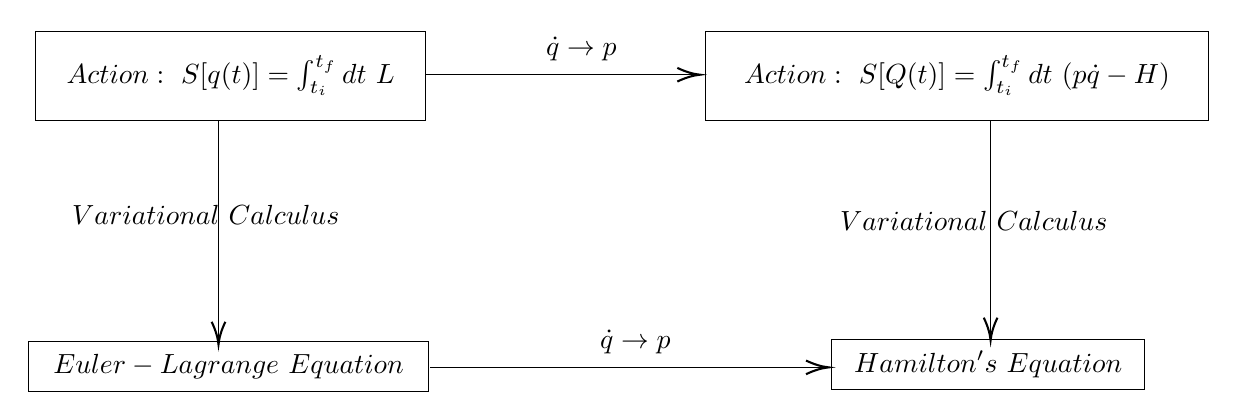
\begin{tikzpicture}[x=0.75pt,y=0.75pt,yscale=-1,xscale=1]
%uncomment if require: \path (0,300); %set diagram left start at 0, and has height of 300

%Straight Lines [id:da8998412978689948] 
\draw    (199.17,49.47) -- (329.17,49.47) ;
\draw [shift={(331.17,49.47)}, rotate = 180] [color={rgb, 255:red, 0; green, 0; blue, 0 }  ][line width=0.75]    (10.93,-3.29) .. controls (6.95,-1.4) and (3.31,-0.3) .. (0,0) .. controls (3.31,0.3) and (6.95,1.4) .. (10.93,3.29)   ;

%Straight Lines [id:da28118020162887525] 
\draw    (99.17,71.47) -- (99.17,177.47) ;
\draw [shift={(99.17,179.47)}, rotate = 270] [color={rgb, 255:red, 0; green, 0; blue, 0 }  ][line width=0.75]    (10.93,-3.29) .. controls (6.95,-1.4) and (3.31,-0.3) .. (0,0) .. controls (3.31,0.3) and (6.95,1.4) .. (10.93,3.29)   ;

%Straight Lines [id:da2698264444244326] 
\draw    (201.17,190.47) -- (391.17,190.47) ;
\draw [shift={(393.17,190.47)}, rotate = 180] [color={rgb, 255:red, 0; green, 0; blue, 0 }  ][line width=0.75]    (10.93,-3.29) .. controls (6.95,-1.4) and (3.31,-0.3) .. (0,0) .. controls (3.31,0.3) and (6.95,1.4) .. (10.93,3.29)   ;

%Straight Lines [id:da134942784322725] 
\draw    (471.17,71.47) -- (471.17,175.47) ;
\draw [shift={(471.17,177.47)}, rotate = 270] [color={rgb, 255:red, 0; green, 0; blue, 0 }  ][line width=0.75]    (10.93,-3.29) .. controls (6.95,-1.4) and (3.31,-0.3) .. (0,0) .. controls (3.31,0.3) and (6.95,1.4) .. (10.93,3.29)   ;


% Text Node
\draw    (11,28.5) -- (199,28.5) -- (199,71.5) -- (11,71.5) -- cycle  ;
\draw (105,50) node    {$Action:\ S[ q( t)] =\int ^{t_{f}}_{t_{i}} dt\ L$};
% Text Node
\draw (274,37) node    {$\dot{q}\rightarrow p$};
% Text Node
\draw    (334,28.5) -- (576,28.5) -- (576,71.5) -- (334,71.5) -- cycle  ;
\draw (455,50) node    {$Action:\ S[ Q( t)] =\int ^{t_{f}}_{t_{i}} dt\ ( p\dot{q} -H)$};
% Text Node
\draw    (7.5,178) -- (200.5,178) -- (200.5,202) -- (7.5,202) -- cycle  ;
\draw (104,190) node    {$Euler-Lagrange\ Equation$};
% Text Node
\draw    (394.5,177) -- (545.5,177) -- (545.5,201) -- (394.5,201) -- cycle  ;
\draw (470,189) node    {$Hamilton's\ Equation$};
% Text Node
\draw (93,117) node    {$Variational\ Calculus$};
% Text Node
\draw (300,178) node    {$\dot{q}\rightarrow p$};
% Text Node
\draw (463,120) node    {$Variational\ Calculus$};


\end{tikzpicture}

\end{center}
\end{qt}


\subsection{Meaning of Hamilton's Equation}
First of all, \textbf{we need to calculate the momentum explicitly:}
$$
\begin{aligned}
p & \equiv \frac{\partial L}{\partial \dot{q}} \\
&=\frac{\partial\left(\frac{1}{2} m \dot{q}^{2}-V(q)\right)}{\partial \dot{q}} \\
&=m \dot{q}
\end{aligned}
$$
Using this result, we ca derive the Hamiltonian:
$$
\begin{aligned}
H &=p \dot{q}-L \\
&=p \dot{q}-\left(\frac{1}{2} m \dot{q}^{2}-V(q)\right) \\
&=p \frac{p}{m}-\left(\frac{1}{2} m\left(\frac{p}{m}\right)^{2}-V(q)\right) \\
&=\frac{p^{2}}{2 m}+V(q)
\end{aligned}
$$
This is exactly the total energy of the object.\redp{The Hamiltonian represents the total energy.}

From the first Hamilton's equation, we have
$$
\begin{aligned}
\frac{d p}{d t} &=-\frac{\partial H}{\partial q} \\
&=-\frac{\partial\left(\frac{p^{2}}{2 m}+V(q)\right)}{\partial q} \\
&=-\frac{\partial V(q)}{\partial q}
\end{aligned}
$$
That is, \redp{The rate of change of momentum equals the force}.

Hamilton's second equation reads:
$$
\begin{aligned}
\frac{d q}{d t} &=\frac{\partial H}{\partial p} \\
&=\frac{\partial\left(\frac{1}{2} \frac{p^{2}}{m}+V(q)\right)}{\partial p} \\
&=\frac{p}{m}
\end{aligned}
$$
Therefore, we can now understand that \redp{the purpose of Hamilton’s second law is to establish a relationship between the momentum and the rate of change of the position}.

\subsection{Hamilton's General Equation}
First of all, we can imagine that sometimes we are not only interested in the locations and momenta of the various objects in
the system but other quantities too. For instance, the temperature or how the kinetic energy evolves as time passes can be interesting things to investigate. \redp{In phase space, the quantities like the temperature or kinetic energy are functions of $q_i$ and $p_i$.}

\begin{mybox}
But how can we calculate the time evolution of such functions depending on the locations $q_{i}(t)$ and momenta $p_{i}(t) ?$
\end{mybox}
For simplicity, let's restrict ourselves to one object moving in one dimension. Then the total rate of change of a function $F=$ $F(q(t), p(t))$ along a single object's trajectory reads:
$$
\frac{d}{d t} F(q, p)=\frac{\partial F(q, p)}{\partial q} \frac{d q}{d t}+\frac{\partial F(q, p)}{\partial p} \frac{d p}{d t}
$$
Using Hamilton's equations, we can write:
$$
\begin{aligned}
\frac{d}{d t} F(q, p) &=\frac{\partial F(q, p)}{\partial q} \frac{d q}{d t}+\frac{\partial F(q, p)}{\partial p} \frac{d p}{d t} \\
&=\frac{\partial F(q, p)}{\partial q} \frac{\partial H(q, p)}{\partial p}-\frac{\partial F(q, p)}{\partial p} \frac{\partial H(q, p)}{\partial q}
\end{aligned}
$$
since the structure that appears on the right-hand side here is so important, it is conventional to introduce a more compact notation. We therefore introduce the \textbf{Poisson bracket $\{,\}$ of two phase space functions $A(q, p), B(q, p)$ by defining}:
\begin{qt}
    \begin{equation}
        \{A, B\} \equiv \frac{\partial A}{\partial q} \frac{\partial B}{\partial p}-\frac{\partial A}{\partial p} \frac{\partial B}{\partial q}
    \end{equation}
\end{qt}
This means that you can’t combine two functions in phase space which describe properties of our system arbitrarily and expect to get something that describes another useful property of
the system. But \textbf{if you calculate the Poisson bracket of the two functions, you’ll get something sensible.} 

Thus, the equation
\begin{qt}
    \begin{equation}
\frac{d}{d t} F=\{F, H\}
\end{equation}
\end{qt}
describes the time evolution of a general phase spack function and we call it \textbf{Hamilton's equation of motion.}

Notice that
\begin{qt}
    $$
\begin{aligned}
\frac{d}{d t} q &=\{q, H\} \\
&=\frac{\partial q}{\partial q} \frac{\partial H}{\partial p}-\frac{\partial q}{\partial p} \frac{\partial H}{\partial q} \\
&=\frac{\partial H}{\partial p}
\end{aligned}
$$
\end{qt}
and
\begin{qt}
    $$
\begin{aligned}
\frac{d}{d t} p &=\{p, H\} \\
&=\frac{\partial p}{\partial q} \frac{\partial H}{\partial p}-\frac{\partial p}{\partial p} \frac{\partial H}{\partial q} \\
&=-\frac{\partial H}{\partial q}
\end{aligned}
$$
\end{qt}
\redp{\textbf{So one way to understand Hamilton's general equation of motion is by imagining that we have a new kind of object $\{, H\}$ (an operator) which eats any function $F$ on phase space $(\{F, H\})$ and spits out the correct time evolution of $F$.}}
\begin{qt}
\begin{center}
    \textbf{The Hamiltonian generates time evolution in phase space.}
\end{center}
\end{qt}
Sometimes we are déaling with a function in phase space which not only depends on $q$ and $p,$ but also explicitly on $t .$ For example, this is necessarily the case if there is a time-dependent potential $V=V(q, t) .$ The total rate of change then reads:
\begin{equation}
\frac{d}{d t} F(q, p, t)=\frac{d q}{d t} \frac{\partial F}{\partial q}+\frac{d p}{d t} \frac{\partial F}{\partial p}+\frac{\partial F}{\partial t}
\end{equation}
In other words,
\begin{qt}
\begin{equation}
\frac{d}{d t} F(q, p, t)=\{F, H\}+\frac{\partial F}{\partial t}
\end{equation}
\end{qt}

\section{The Newtonian Algorithm}
\begin{mybox}
We stand at the top of the Leaning Tower of Pisa and let a ball fall to the ground. How is the ball moving?
\end{mybox}
$$
\vec{F}=\left(\begin{array}{r}
{0} \\
{0} \\
{-m g}
\end{array}\right)
$$
Newton's second law tells us
$$
\begin{aligned}
\frac{d \vec{p}}{d t} &=\vec{F} \\
\frac{d(m \vec{v})}{d t} &=\left(\begin{array}{r}
{0} \\
{0} \\
{-m g}
\end{array}\right) \\
m \frac{d}{d t}\left(\begin{array}{l}
{v_{x}} \\
{v_{z}}
\end{array}\right) &=\left(\begin{array}{r}
{0} \\
{-m g}
\end{array}\right) \\
\frac{d}{d t}\left(\begin{array}{l}
{v_{x}} \\
{v_{z}}
\end{array}\right) &=\left(\begin{array}{r}
{0} \\
{-g}
\end{array}\right)
\end{aligned}
$$
Our task is to solve these three equations of motion. Luckily, we can simply integrate the equations twice since gravity is constant:
$$
\begin{aligned}
\frac{d}{d t}\left(\begin{array}{c}
{v_{x}} \\
{v_{y}} \\
{v_{z}}
\end{array}\right) &=\left(\begin{array}{c}
{0} \\
{0} \\
{-g}
\end{array}\right) \\
\int_{0}^{t} d t^{\prime} \frac{d}{d t^{\prime}}\left(\begin{array}{c}
{v_{x}} \\
{v_{y}} \\
{v_{z}}
\end{array}\right) &=\int_{0}^{t} d t^{\prime}\left(\begin{array}{c}
{0} \\
{-g}
\end{array}\right) \\
\left(\begin{array}{c}
{v_{x}(t)} \\
{v_{z}(t)}
\end{array}\right)-\left(\begin{array}{c}
{v_{x}(0)} \\
{v_{z}(0)}
\end{array}\right)=\left(\begin{array}{c}
{0} \\
{0} \\
{-g t}
\end{array}\right)
\end{aligned}
$$
$\int_{0}^{t} d t^{\prime}\left(\begin{array}{l}{v_{x}\left(t^{\prime}\right)} \\ {v_{y}\left(t^{\prime}\right)} \\ {v_{z}\left(t^{\prime}\right)}\end{array}\right)-\int_{0}^{t} d t^{\prime}\left(\begin{array}{l}{v_{x}(0)} \\ {v_{y}(0)} \\ {v_{z}(0)}\end{array}\right)=\int_{0}^{t} d t^{\prime}\left(\begin{array}{c}{0} \\ {0} \\ {-g t}\end{array}\right)$
$$
\left(\begin{array}{l}
{x(t)} \\
{y(t)} \\
{z(t)}
\end{array}\right)-\left(\begin{array}{l}
{x(0)} \\
{y(0)} \\
{z(0)}
\end{array}\right)-\left(\begin{array}{l}
{v_{x}(0) t} \\
{v_{y}(0) t} \\
{v_{z}(0) t}
\end{array}\right)=\left(\begin{array}{c}
{0} \\
{0} \\
{-\frac{1}{2} g t^{2}}
\end{array}\right)
$$
Next, we need to determine the integration constants
$$
v_{x}(0), v_{y}(0), v_{z}(0), x(0), y(0), z(0)
$$
Let
$$
\left(\begin{array}{l}
{v_{x}(0)} \\
{v_{y}(0)} \\
{v_{z}(0)}
\end{array}\right)=\left(\begin{array}{l}
{0} \\
{0} \\
{0}
\end{array}\right)
$$
$$
\left(\begin{array}{l}
{x(0)} \\
{y(0)} \\
{z(0)}
\end{array}\right)=\left(\begin{array}{l}
{0} \\
{0} \\
{0}
\end{array}\right)
$$
Finally
$$
\left(\begin{array}{c}
{x(t)} \\
{y(t)} \\
{z(t)}
\end{array}\right)=\left(\begin{array}{c}
{0} \\
{0} \\
{-\frac{1}{2} g t^{2}}
\end{array}\right)
$$
\section{Lagrangian Algorithm}
\begin{mybox}
We stand at the top of the Leaning Tower of Pisa and let a ball fall to the ground. How is the ball moving?
\end{mybox}
The Lagrangian reads
$$
\begin{aligned}
L=T-V &=\frac{1}{2} m \vec{v}^{2}-m g z \\
&=\frac{1}{2} m\left(v_{x}^{2}+v_{y}^{2}+v_{z}^{2}\right)-m g z
\end{aligned}
$$
Since $\frac{\partial L}{\partial q}=\frac{d}{d t}\left(\frac{\partial L}{\partial v_{q}}\right)$,
$$
0=m \frac{d}{d t} v_{x}
$$
$$
0=m \frac{d}{d t} v_{y}
$$
$$
-m g=m \frac{d}{d t} v_{z}
$$
\textbf{Take note that in the derivations above, we didn’t have to think about vectors at all. This is one advantage of the Lagrangian formalism.} In addition, the Lagrangian formulation of classical mechanics is always a good choice whenever we are dealing with a system which is subject to constraints.

\subsection{Constraints}
In mathematical terms, a constraint is a relationship between coordinates. For example, for a mass attached to a circular loop with radius $l,$ we have the constraint
$$
x^{2}+y^{2}=l^{2}
$$
More generally, a \textbf{holonomic constraint} is a formula of the form
$$
f\left(q, 1, q_{2}, \ldots, t\right)=\text { const. }
$$
\begin{qt}
\textbf{Non-holonomic constraints}
$$
f\left(q_{1}, 1, q_{2}, \ldots\right) \geq \text { const. }
$$
$$
f(q, \dot{q}, t)=\text { const. }
$$
Additionally, take note that it is conventional to call a constraint which does not explicitly depend on $t$ scleronomic (Greek for "rigid") and a constraint with explicit dependence on $t$ rheonomic (Greek for "moving").
\end{qt}
The trick which allows us to incorporate constraints in the Lagrangian formalism is known as the method of \textbf{Lagrange multipliers} and works as follows.
\begin{mybox}
\begin{center}
    How to use Lagrange multiplier to add a holonomic constraint?
\end{center}
\end{mybox}
\begin{mybox2}
First, we rewrite the constraint as:
$$
g\left(q_{1}, 1, q_{2}, \ldots, t\right) \equiv f\left(q_{1}, 1, q_{2}, \ldots, t\right)-\text { const. }
$$
We then take the Lagrangian $L_{\text {free that we would use if the }}$ object could move around freely without constraints and add a new term $L_{\text {con}}$  which encodes the constraint 
$$
\begin{aligned}
L_{\text {full }} &=L_{\text {free }}+L_{\text {con }} \\
&=L_{\text {free }}+\lambda g(q, t)
\end{aligned}
$$
If we treat $\lambda$ as a new coordinate, the Euler-Lagrange equation for $\lambda$ tells us
$$
\begin{array}{c}
{\frac{\partial L}{\partial \lambda}=\frac{d}{d t}\left(\frac{\partial L}{\partial \dot{\lambda}}\right)} \\
{\frac{\partial\left(L_{\text {free }}+\lambda g(q, t)\right)}{\partial \lambda}=\frac{d}{d t}\left(\frac{\partial\left(L_{\text {free }}+\lambda g(q, t)\right)}{\partial \lambda}\right)} \\
{\frac{\partial(\lambda g(q, t))}{\partial \lambda}=\frac{d}{d t}\left(\frac{\partial(\lambda g(q, t))}{\partial \dot{\lambda}}\right)} \\
{\frac{\partial(\lambda g(q, t))}{\partial \lambda}=0} \\
{g(q, t)=0}
\end{array}
$$
In addition, by using the Euler-Lagrange equation for our ordinary coordinates $q,$ we find
$$
\begin{aligned}
\frac{\partial L}{\partial q} &=\frac{d}{d t}\left(\frac{\partial L}{\partial \dot{q}}\right) \\
\frac{\partial\left(L_{\text {free }}+\lambda g(q, t)\right)}{\partial q} &=\frac{d}{d t}\left(\frac{\partial\left(L_{\text {free }}+\lambda g(q, t)\right)}{\partial \dot{q}}\right) \\
\frac{\partial\left(L_{\text {free }}+\lambda g(q, t)\right)}{\partial q} &=\frac{d}{d t}\left(\frac{\partial L_{\text {free }}}{\partial \dot{q}}\right) \\
\frac{\partial L_{\text {free }}}{\partial q}+\lambda \frac{\partial g(q, t)}{\partial q} &=\frac{d}{d t}\left(\frac{\partial L_{\text {free }}}{\partial \dot{q}}\right)
\end{aligned}
$$
we've learned that the term on the right-hand side $\frac{d}{d t}\left(\frac{\partial L_{\text {free }}}{\partial q}\right)$ is analogous to $\frac{d p}{d t}$ in the Newtonian formalism. Moreover, the first term on the left-hand side $\frac{\partial L_{\text {free }}}{\partial q}$ describes the forces. In other words, $\lambda \frac{\partial g(q, t)}{\partial q}$ add new forces to the equation of motion.
\end{mybox2}
If there is more than one constraint
$$
L_{\text {full }}=L_{\text {free }}+\lambda_{1 g_{1}}(q, t)+\lambda_{2} g_{1}(q, t)+\ldots
$$
Moreover, using the Euler-Lagrange equation for the regular coordinate $q$ yields the equation of motion including all constraint forces:
$$
\frac{\partial L_{\text {free }}}{\partial q}+\lambda_{1} \frac{\partial g_{1}(q, t)}{\partial q}+\lambda_{2} \frac{\partial g_{2}(q, t)}{\partial q}+\ldots=\frac{d}{d t}\left(\frac{\partial L_{\text {free }}}{\partial \dot{q}}\right)
$$

\subsection{Point Transformations and Generalized Coordinates}
In general, we call a transformation from one set of coordinates in configuration space $q=\left(q_{1}, q_{2}, \ldots\right)$ to a new set of coordinates $q^{\prime}=\left(q_{1}^{\prime}, q_{2}^{\prime}, \ldots\right)$ a\textbf{ point transformation.}

\chapter{Quantum Mechaaaaanics}
\chapter{Electromagnetism}
\section{Fundamental Concepts}
\subsection{Charge, Current, Flux}
\begin{qt}
    \begin{center}
        Electric charge is conserved no matter how small our system is, even for elementary particle processes
    \end{center}
\end{qt}
\begin{qt}
    The total charge inside any volume $V$ is then given by the integral over the charge density:
    \begin{equation}
Q=\int_{V} d^{3} x \rho(\vec{x}, t)
\end{equation}
\end{qt}
Of course, \textbf{we can also use the charge density if there is only one charged object in our system.} In this case, the charge density is zero everywhere except at one specific point. Any integral over a region which contains the location of the object, yields simply the charge of the object. 
\begin{qt}
    Specifically, the charge density of a system with just one charged object located at $\vec{x}_{0}$ is
    \begin{equation}
\rho(\vec{x})=q \delta\left(\vec{x}-\vec{x}_{0}\right)
\end{equation}
\end{qt}
where $q$ is the charge of the object. Any integral over a region $V_{0}$ which contains $\vec{x}_{0}$ yields exactly $q,$ as it should be
$$
\begin{aligned}
\int_{V_{0}} d^{3} x \rho(\vec{x}, t) &=\int_{V_{0}} d^{3} x q \delta\left(\vec{x}-\vec{x}_{0}\right) \\
&=q \int_{V_{0}} d^{3} x \delta\left(\vec{x}-\vec{x}_{0}\right) \\
&=q
\end{aligned}
$$
\begin{qt}
    In electrodynamics, the \redp{the electric current} is defined as:
    \begin{equation}
I=\frac{d Q}{d t}
\end{equation}
\end{qt}
The correct tool to describe the flow of charges in three dimensions is called \textbf{\redp{current density}}. \bluep{A current density yields a vector at each point in space(i.e., vector space). The direction of the vector at a given point describes the direction of the flow. The length of the vector describes how much is flowing.}
\begin{qt}
    By introducing a vector $\vec{n}$ of unit length normal to a frame with area of $A$, we can calculate the current passing through the frame as:
    \begin{equation}
I \equiv \frac{\Delta Q}{\Delta t}=\rho_{0} A \vec{v}_{c} \cdot \vec{n}
\end{equation}
If we define \textbf{\redp{the electric current density}} as 
\begin{equation}
\vec{J} \equiv \rho_{0} \vec{v}_{c}
\end{equation}
we have
\begin{equation}
\vec{J} \cdot \vec{n} A=\rho_{0} \vec{v}_{c} \cdot \vec{n} A=I
\end{equation}
\end{qt}
In general, \textbf{the magnitude of the current density $|\vec{J}|$ at one specific point describes the amount of electric charge which passes per unit time through an infinitesimal surface element which is at right angles to the direction of the flow.} The direction of the charge density vector $\vec{J}$ encodes where the charges are flowing.

\begin{qt}
    If we want to know how much electric charge is flowing through a more complicated surface $S$, we have to calculate the \textbf{\redp{surface integral}}:
    \begin{equation}
I=\int_{S} \vec{J} \cdot \overrightarrow{d S}
\end{equation}
The total amount of charge passing through the surface $S$ during some time interval $\Delta t$ is then given by
\begin{equation}
\Delta Q=\Delta t \int_{S} \vec{J} \cdot \overrightarrow{d S}
\end{equation}
\end{qt}

\subsection{Electromagnetic Field}
An important feature of the electromagnetic field is that even a vector field is not sufficient and we need instead a tensor field. \textbf{The electromagnetic field tensor is an antisymmetric $(4 \times 4)$ matrix}
\begin{qt}
    \begin{equation}
F_{\mu \nu}(t, \vec{x})=\left(\begin{array}{cccc}
{0} & {F_{01}(t, \vec{x})} & {F_{02}(t, \vec{x})} & {F_{03}(t, \vec{x})} \\
{-F_{01}(t, \vec{x})} & {0} & {F_{12}(t, \vec{x})} & {F_{13}(t, \vec{x})} \\
{-F_{02}(t, \vec{x})} & {-F_{12}(t, \vec{x})} & {0} & {F_{23}(t, \vec{x})} \\
{-F_{03}(t, \vec{x})} & {-F_{13}(t, \vec{x})} & {-F_{23}(t, \vec{x})} & {0}
\end{array}\right)
\end{equation}
\redp{This tensor field, in some sense, assigns exactly two vectors to each point in space $\vec{x}$ at each point in time $t .$ }
\end{qt}
The vectors at each location represent the strength and direction of the electromagnetic field. It is conventional to introduce the electric vector field $\vec{E}(t, \vec{x})$ and the magnetic vector field $\vec{B}(t, \vec{x})$ and work with them, instead of with the electromagnetic tensor field $F_{\mu \nu}(t, \vec{x})$.
\begin{equation}
F_{\mu \nu}(t, \vec{x})\equiv\left(\begin{array}{cccc}
{0} & {-E_{1}(t, \vec{x}) / c} & {-E_{2}(t, \vec{x}) / c} & {-E_{3}(t, \vec{x}) / c} \\
{E_{1}(t, \vec{x}) / c} & {0} & {-B_{3}(t, \vec{x})} & {B_{2}(t, \vec{x})} \\
{E_{2}(t, \vec{x}) / c} & {B_{3}(t, \vec{x})} & {0} & {-B_{1}(t, \vec{x})} \\
{E_{3}(t, \vec{x}) / c} & {-B_{2}(t, \vec{x})} & {B_{1}(t, \vec{x})} & {0}
\end{array}\right)
\end{equation}
\bluep{Each of these two fields $\vec{E}(t, \vec{x})=\left(E_{1}(t, \vec{x}), E_{2}(t, \vec{x}), E_{3}(t, \vec{x})\right)^{T}$
and $\vec{B}(t, \vec{x})=\left(B_{1}(t, \vec{x}), B_{2}(t, \vec{x}), B_{3}(t, \vec{x})\right)^{T}$ assigns a vector to each point in space $\vec{x}$ at each point in time $t$}.

Unfortunately, the interpretation of the electric field $\vec{E}(t, \vec{x})$ and the magnetic field $\vec{B}(t, \vec{x})$ is not so simple. Instead, the little arrows encode information about the somewhat abstract "physical field", which we can understand as follows: \redp{The direction of the vector at a given location encodes in which direction a test charge would move if it were placed here. The magnitude of the vector encodes how fast the test charge would accelerate as a result of, for example, the electric field}. In this sense, these more abstract fields encode how something would
flow if it were there.
\begin{qt}
    In practice the electric field strength at a point is measured by placing a small test charge at that point and measuring the force on it:
    \begin{equation}
\vec{E}(\vec{x}) \equiv \frac{\vec{F}(\vec{x})}{q}
\end{equation}
\end{qt}
\subsection{Electromagnetic potential}
For the moment, we only note that the electromagnetic potential is characterized by 4 numbers at each point in space and time $A_{\mu}(t, \vec{x})=\left(A_{0}(t, \vec{x}), A_{1}(t, \vec{x}), A_{2}(t, \vec{x}), A_{3}(t, \vec{x})\right)^{T}$ and that the electric and magnetic fields can be calculated immediately once the electromagnetic potential is specified:
\begin{qt}
    \begin{equation}
\begin{aligned}
&E_{i}=\left(-\partial_{i} A_{0}-\partial_{0} A_{i}\right) / c\\
&B_{i}=\epsilon_{i j k} \partial_{j} A_{k}
\end{aligned}
\end{equation}
where $i, j, k \in\{1,2,3\} .$ We can also write this as a vector equations
\begin{equation}
\begin{aligned}
&\vec{E}=\left(-\nabla A_{0}-\partial_{t} \vec{A}\right) / c\\
&\vec{B}=\nabla \times \vec{A}
\end{aligned}
\end{equation}
\end{qt}
We can also express the tensor field itself using the electromagnetic potential
\begin{qt}
    \begin{equation}
F_{\mu v}=\partial_{\mu} A_{v}-\partial_{v} A_{\mu}
\end{equation}
\end{qt}

\section{Fundamental Equations}

\chapter{Tensor Calculus}

\section{Total and Partial Derivatives}
To understand the different kinds of derivatives, let's say we have a function $\rho(t, x(t), p(t))$ which, in general, depends on the location $x(t)$ and momentum $p(t)$ plus the time $t.$ A key observation is that the location $x(t)$ and momentum $p(t)$ are functions of $t$ too. Therefore, we need to be extremely careful what we mean when we calculate the derivative with respect to the time $t .$
$$
\frac{d \rho}{d t}=\lim _{\Delta t \rightarrow 0} \frac{\rho(t+\Delta t, x(t+\Delta t), p(t+\Delta t))-\rho(t, x(t), p(t))}{\Delta t}
$$
\textbf{The result is the total rate of change of $\rho$}.
$$
\frac{\partial \rho}{\partial t}=\lim _{\Delta t \rightarrow 0} \frac{\rho(t+\Delta t, x(t), p(t))-\rho(t, x(t), p(t))}{\Delta t}
$$
The key difference is that we only vary $t$ if it appears explicitly
in $\rho$ but not if it only appears implicitly because $x(t)$ and $p(t)$
also depend on $t .$ Thus
$$
\frac{d \rho}{d t}=\frac{\partial \rho}{\partial x} \frac{d x}{d t}+\frac{\partial \rho}{\partial p} \frac{d p}{d t}+\frac{\partial \rho}{\partial t}
$$
\section{Taylor Expansion}
In general, we want to estimate the value of some function $f(x)$ at some value of $x$ by using our knowledge of the function's value at some fixed point $a .$ The Taylor series then reads
\begin{equation}
\begin{aligned}
f(x)=& \sum_{n=0}^{\infty} \frac{f^{(n)}(a)(x-a)^{n}}{n !} \\
=& \frac{f^{(0)}(a)(x-a)^{0}}{0 !}+\frac{f^{(1)}(a)(x-a)^{1}}{1 !}+\frac{f^{(2)}(a)(x-a)^{2}}{2 !} \\
&+\frac{f^{(3)}(a)(x-a)^{3}}{3 !}+\ldots
\end{aligned}
\end{equation}
or
\begin{equation}
f(x+a)=f(x)+(a \cdot \partial) f(x)+\frac{1}{2}(a \cdot \partial)^{2} f(x)+\cdots
\end{equation}
Taylor expansion of a scalar field (function $f$ that maps $\mathbb{R}^{n}$ to $\mathbb{R}$).Now, identify $\partial f / \partial t$ as $\hat{\boldsymbol{n}} \cdot \nabla f .$ In addition, see that $t \hat{\boldsymbol{n}}=\boldsymbol{x}-\boldsymbol{x}_{0} .$ Some clever recombining of terms gives
\begin{equation}
f(x)=f\left(x_{0}\right)+\left.\left(x-x_{0}\right) \cdot \nabla f\right|_{x_{0}}+\left.\frac{1}{2}\left(\left[x-x_{0}\right] \cdot \nabla\right)^{2} f\right|_{x_{0}}+\ldots
\end{equation}
and
\begin{equation}
\hat{\boldsymbol{n}} \cdot \nabla=\partial_{t}
\end{equation}

\section{Vector Identities}
\begin{equation}
\begin{aligned}
&\vec{\nabla} \cdot(\vec{\nabla} \times \vec{A}) \equiv \operatorname{div}(\operatorname{rot} \vec{A})=(\vec{\nabla} \times \vec{\nabla}) \cdot \vec{A} \equiv 0\\
&\vec{\nabla} \times(\vec{\nabla} \varphi) \equiv \operatorname{rot} \operatorname{grad} \varphi=(\vec{\nabla} \times \vec{\nabla}) \varphi \equiv 0
\end{aligned}
\end{equation}
\begin{equation}
\begin{aligned}
&\vec{\nabla} \cdot(\vec{A} \varphi)=\varphi \vec{\nabla} \cdot \vec{A}+\vec{A} \cdot \vec{\nabla} \varphi \quad \Longleftrightarrow \quad \operatorname{div}(\vec{A} \varphi)=\varphi \operatorname{div} \vec{A}+\vec{A} \cdot \operatorname{grad} \varphi\\
&\vec{\nabla} \times(\vec{A} \varphi)=\varphi \vec{\nabla} \times \vec{A}-\vec{A} \times \vec{\nabla} \varphi \quad \Longleftrightarrow \quad \operatorname{rot}(\vec{A} \varphi)=\varphi \operatorname{rot} \vec{A}-\vec{A} \times \operatorname{grad} \varphi\\
&\vec{\nabla} \cdot(\vec{A} \times \vec{B})=\vec{B} \cdot(\vec{\nabla} \times \vec{A})-\vec{A} \cdot(\vec{\nabla} \times \vec{B}) \quad \Longleftrightarrow \quad \operatorname{div}(\vec{A} \times \vec{B})=\vec{B} \cdot \operatorname{rot} \vec{A}-\vec{A} \cdot \operatorname{rot} \vec{B}
\end{aligned}
\end{equation}
\begin{equation}
\begin{aligned}
\vec{\nabla} \times(\vec{A} \times \vec{B}) &=(\vec{B} \cdot \vec{\nabla}) \vec{A}-(\vec{A} \cdot \vec{\nabla}) \vec{B}+\vec{A}(\vec{\nabla} \cdot \vec{B})-\vec{B}(\vec{\nabla} \cdot \vec{A}) \\
& \Longleftrightarrow \operatorname{rot}(\vec{A} \times \vec{B})=(\vec{B} \operatorname{grad}) \vec{A}-(\vec{A} \operatorname{grad}) \vec{B}+\vec{A}(\operatorname{div} \vec{B})-\vec{B}(\operatorname{div} \vec{A})
\end{aligned}
\end{equation}
\begin{equation}
\begin{aligned}
\vec{\nabla}(\vec{A} \cdot \vec{B})=&(\vec{B} \cdot \vec{\nabla}) \vec{A}+(\vec{A} \cdot \vec{\nabla}) \vec{B}+\vec{A} \times(\vec{\nabla} \times \vec{B})+\vec{B} \times(\vec{\nabla} \times \vec{A}) \\
& \Longleftrightarrow \operatorname{grad}(\vec{A} \cdot \vec{B})=(\vec{B} \cdot \operatorname{grad}) \vec{A}+(\vec{A} \cdot \operatorname{grad}) \vec{B}+\vec{A} \times \operatorname{rot} \vec{B}+\vec{B} \times \operatorname{rot} \vec{A}
\end{aligned}
\end{equation}
\begin{equation}
\begin{aligned}
&\vec{\nabla} \cdot(\vec{\nabla} \varphi) \equiv \operatorname{div}(\operatorname{grad} \varphi) \equiv \Delta \varphi=\frac{\partial^{2} \varphi}{\partial x^{2}}+\frac{\partial^{2} \varphi}{\partial y^{2}}+\frac{\partial^{2} \varphi}{\partial z^{2}}, \quad \Delta=\text { Laplace Operator }\\
&\vec{\nabla} \times(\vec{\nabla} \times \vec{A}) \equiv \operatorname{rot}(\operatorname{rot} \vec{A})=\vec{\nabla}(\vec{\nabla} \cdot \vec{A})-(\vec{\nabla} \cdot \vec{\nabla}) \vec{A} \equiv \operatorname{grad} \operatorname{div} \vec{A}-\Delta \vec{A}
\end{aligned}
\end{equation}

\section{Linear Spaces, Vectors, and Tensors}
The linear space, say $L$, consists of the elements (vectors) that \textbf{permit linear operations with the properties described below}:
\begin{itemize}
    \item Summing up the vectors
    \item Multiplication by a number
\end{itemize}
\begin{qt}
    Consider the set of vectors, elements of the linear space L
    $$
\left\{\mathbf{a}_{1}, \mathbf{a}_{2}, \ldots, \mathbf{a}_{n}\right\}=\left\{\mathbf{a}_{i} | i=1, \ldots, n\right\}
$$
and the set of real numbers $k_{1}, k_{2}, \ldots k_{n} .$ Vector
$$
\mathbf{k}=\sum_{i=1}^{n} k^{i} \mathbf{a}_{i}=\mathbf{k}^{i} \mathbf{a}_{i}=0\Longrightarrow \sum_{i=1}^{n}\left(k^{i}\right)^{2}=0
$$
then vectors $\left\{\mathbf{a}_{\mathbf{i}}, i=1, \ldots, n\right\}$ are called \textbf{linearly independent}. The last condition means that no one of the coefficients $k_{i}$ can be different from zero.
\end{qt}
For example, in 2D, two vectors are linearly dependent if and only if they are parallel; in 3D, three vectors are linearly dependent if and only if they belong to the same plane, etc.
\begin{defi}
        The maximal number of linearly independent elements of the linear space $L$ is called its dimension. It proves useful to denote $L_{D}$ a linear space of dimension $D .$
\end{defi}
\begin{thm}
Consider a $D$-dimensional linear space $L_{D}$ and the set of linearly independent vectors $\mathbf{e}_{i}=\left(\mathbf{e}_{1}, \mathbf{e}_{2}, \ldots, \mathbf{e}_{D}\right) .$ Then, for any vector a one can write
\begin{equation}
    \mathbf{a}=\sum_{i=1}^{D} a^{i} \mathbf{e}_{i}=a^{i} \mathbf{e}_{i}
    \label{vector-basis}
\end{equation}
where the coefficients $a^{i}$ are defined in a unique way.
\end{thm}
\bluep{The coefficients $a^{i}$ are called components or \textbf{contravariant components of the vector $\mathbf{a}$}}.The word “contravariant” here means that the components $a^i$ have upper indices.

\section{Direct product of the two linear spaces}
Let's consider the example of phase space in the classic mechanics. The coordinate system in the linear space $L_{D}$ consists of the initial point $O$ and the basis $\mathbf{e}_{i} .$ The position of a point $P$ can be characterized by \textbf{its position vector or radius vector $\mathbf{r}=\overrightarrow{O P}=x^{i} \mathbf{e}_{i}$}.

If the phase space is describing one particle, the space is composed of the radius vectors $\mathbf{r}$ and velocities $\mathbf{v}$ of the particle:
$$
\mathbf{r}=x^{i} \mathbf{e}_{i}, \quad \mathbf{v}=v^{j} \mathbf{f}_{j}
$$
The two set of bases can be related and independent. This example is a particular case of the linear space which is called \redp{a direct product
of the two linear spaces}. The element of the direct product of the two linear spaces $L_{D_{1}}$ and $L_{D_{2}}$ (\textbf{they can have different dimensions}) is the ordered set of the elements of each of the two spaces $L_{D_{1}}$ and $L_{D_{2}} .$
\begin{qt}
    The notation for the basis in the case of configuration space is $\mathbf{e}_{i} \otimes \mathbf{f}_{j}$. Hence, the state of the point-like particle in the phase space is characterized by the element of this linear space, which can be presented as:
    $$
x^{i} v^{j} \mathbf{e}_{i} \otimes \mathbf{f}_{j}
$$
In general, one can define the space that is a direct product of several linear spaces with different individual basis sets $\mathbf{e}_{i}$ each. In this case, we will have $\mathbf{e}_{i}^{(1)}, \mathbf{e}_{i}^{(2)}, \ldots$ $\mathbf{e}_{i}^{(N)} .$ The basis in the direct product space will be
$$
\mathbf{e}_{i_{1}}^{(1)} \otimes \mathbf{e}_{i_{2}}^{(2)} \otimes \ldots \otimes \mathbf{e}_{i_{N}}^{(N)}
$$
and the element becomes
$$
T^{i_{1} i_{2} \ldots i_{N}} \mathbf{e}_{i_{1}}^{(1)} \otimes \mathbf{e}_{i_{2}}^{(2)} \otimes \ldots \otimes \mathbf{e}_{i_{N}}^{(N)}
$$
\end{qt}
\section{Vector basis and its transformation}
Let us start from the components of the vector, which were defined in (\ref{vector-basis}). Consider, along with the original basis $\mathbf{e}_{i},$ another basis $\mathbf{e}_{i}^{\prime} .$ since each vector of the new basis belongs to the same space, it can be expanded using the original basis as
\begin{equation}
\mathbf{e}_{i}^{\prime}=\wedge_{i^{\prime}}^{j} \mathbf{e}_{j}
\label{basis-transform}
\end{equation}
and
$$
\mathbf{a}=a^{i} \mathbf{e}_{i}=a^{j^{\prime}} \mathbf{e}_{j^{\prime}}=a^{j^{\prime}} \wedge_{j^{\prime}}^{i} \mathbf{e}_{i}
$$
\begin{qt}
\begin{equation}
    a^{i}=a^{j^{\prime}} \wedge_{j^{\prime}}^{i}
    \label{cotravariant-coord-transform}
\end{equation}
\end{qt}

Similarly, we can make inverse transformation:
$$
a^{k^{\prime}}=\left(\wedge^{-1}\right)_{l}^{k^{\prime}} a^{l}
$$
and
\[
\left(\wedge^{-1}\right)_{l}^{k^{\prime}} \cdot \wedge_{i^{\prime}}^{l}=\delta_{i^{\prime}}^{k^{\prime}} \quad \text { and } \quad \wedge_{i^{\prime}}^{l} \cdot\left(\wedge^{-1}\right)_{k}^{i^{\prime}}=\delta_{k}^{l}
\]
\begin{qt}
Taking the partial derivatives, we arrive at the relations
\[
\wedge_{j^{\prime}}^{i}=\frac{\partial x^{i}}{\partial x^{j^{\prime}}} \quad \text { and } \quad\left(\wedge^{-1}\right)_{l}^{k^{\prime}}=\frac{\partial x^{k^{\prime}}}{\partial x^{l}}
\]
and
$$
\left(\wedge^{-1}\right)_{l}^{k^{\prime}} \cdot \wedge_{k^{\prime}}^{i}=\frac{\partial x^{k^{\prime}}}{\partial x^{l}} \frac{\partial x^{i}}{\partial x^{k^{\prime}}}=\frac{\partial x^{i}}{\partial x^{l}}=\delta_{l}^{i}
$$
is nothing but the chain rule for partial derivatives.
\end{qt}

\section{Scalar, vector, and tensor fields}
\begin{defi}
        Function $\varphi(x)$ is called scalar field or simply scalar if it does not transform under the change of coordinates
        \begin{equation}
\varphi(x)=\varphi^{\prime}\left(x^{\prime}\right)
\end{equation}
\end{defi}
Let us give a clarifying example in 1D. Consider a function
$$
y=x^2
$$
Now, let us change the variables 
$$
x^{\prime}=x+1
$$
The function $y=\left(x^{\prime}\right)^{2},$ obviously, represents another parabola. \bluep{In order to preserve the plot intact, we need to modify the form of the function, that is, to go from $\varphi$ to $\varphi^{\prime}$.} The new function $y^{\prime}=\left(x^{\prime}-1\right)^{2}$ will represent the original parabola,because the change of the variable is completely compensated by the change of the form of the function.
\begin{mybox}
\begin{center}
    Discuss whether the three numbers temperature $T(x)$, pressure $p(x)$ and density $\rho(x)$ form a contravariant vector
\end{center}
\end{mybox}
\begin{mybox2}
We can only form contravariant vector if the numbers transform by following the rule (\ref{cotravariant-coord-transform}). Since these numbers are scalar fields, it transforms like $T(\mathbf{r})=T^{\prime}(\mathbf{r}^{\prime})$. Thus, these three parameters can not form a contravariant vector.
\end{mybox2}
\begin{example}
From the definition above we know $\varphi^{\prime}(x) \neq \varphi(x)$ and $\varphi\left(x^{\prime}\right) \neq \varphi(x)$. Let us calculate these quantities explicitly for the special case of infinitesimal transformation $x^{\prime i}=x^{i}+\xi^{i}$ where $\xi$ are constant coefficients. Now we have
$$
\varphi\left(x^{\prime}\right)=\varphi\left(x+\xi\right)\overset{Taylor}{=}\varphi(x)+\frac{\partial \varphi}{\partial x^{i}} \xi^{i}
$$
and,
$$
\varphi^{\prime}\left(x^{i}\right)=\varphi^{\prime}\left(x^{i}-\xi^{i}\right)=\varphi^{\prime}\left(x^{\prime}\right)-\frac{\partial \varphi^{\prime}}{\partial x^{i^{\prime}}} \cdot \xi^{i}
$$
rewrite the two equations above, we find:
$$
\frac{\partial \varphi^{\prime}}{\partial x^{\prime i}}=\frac{\varphi^{\prime}\left(x^{\prime i}\right)-\varphi^{\prime}\left(x^{i}-\xi^{i}\right)}{\xi^i}
$$
$$
\frac{\partial \varphi}{\partial x^{i}}=\frac{\varphi(x^{\prime i})-\varphi(x^i)}{\xi^i}
$$
At the limit of $\xi\rightarrow0$, we have
$$
\frac{\partial \varphi^{\prime}}{\partial x^{\prime i}}=\frac{\partial \varphi(x)}{\partial x^{i}}+\mathcal{O}(\xi)
$$
As mentioned above, 
$$
\varphi^{\prime}\left(x^{i}\right)=\varphi^{\prime}\left(x^{\prime}\right)-\frac{\partial \varphi^{\prime}}{\partial x^{\prime i}} \cdot \xi^{i}\\
=\varphi^{\prime}\left(x^{\prime}\right)-\frac{\partial \varphi(x)}{\partial x^{i}}\cdot\xi^i
$$
Since $\varphi(x)=\varphi^{\prime}\left(x^{\prime}\right)$, we have
$$
\varphi^{\prime}(x)=\varphi(x)-\xi^{i} \partial_{i} \varphi
$$
\textbf{where we have introduced a useful notation $\partial_{i}=\partial / \partial x^{i}$.}
\end{example}
\textbf{For the vector field, we have the following rule for the coordinate transformation}. The set of three functions $\left\{a^{i}(x)\right\}=\left\{a^{1}(x), a^{2}(x), a^{3}(x)\right\}$ forms contravariant vector field (or simply vector field) if they transform, under the change of coordinates $\left\{x^{i}\right\} \rightarrow\left\{x^{\prime} j\right\},$ as
\begin{qt}
\begin{equation}
a^{j^{\prime}}\left(x^{\prime}\right)=\frac{\partial x^{j^{\prime}}}{\partial x^{i}} \cdot a^{i}(x)
\end{equation}
\end{qt}
\bluep{The components of the vector in a given geometrical point of space modify under the coordinate transformation, while the scalar field does not.}The scalar and vector fields can be considered as examples of the more general objects called tensors. Tensors are also defined through their transformation rules.
\begin{qt}
The set of $3^n$ functions $\left\{a^{i_{1} \ldots i_{n}}(x)\right\}$ is called a contravariant tensor of rank $n,$ if these functions transform, under $x^{i} \rightarrow x^{i},$ as
\begin{equation}
a^{i_{1}^{i} \ldots i_{n}^{\prime}}\left(x^{\prime}\right)=\frac{\partial x^{i_{1}^{\prime}}}{\partial x^{j_{1}}} \ldots \frac{\partial x^{i_{n}^{\prime}}}{\partial x^{j_{n}}} a^{j_{1} \ldots j_{n}}(x)
\end{equation}
\end{qt}

\section{Orthonormal Basis and Cartesian Coordiantes}
The scalar product of two vectors $\mathbf{a}$ and $\mathbf{b}$ in 3D is defined in a ususal way,
\begin{equation}
(\mathbf{a}, \mathbf{b})=\mathbf{a}\cdot\mathbf{b}=|\mathbf{a}| \cdot|\mathbf{b}| \cdot \cos \theta
\end{equation}
Special orthonormal basis $\left\{\hat{\mathbf{n}}_{a}\right\}$ is the one with
\begin{equation}
\left(\hat{\mathbf{n}}_{a}, \hat{\mathbf{n}}_{b}\right)=\delta_{a b}=\left\{\begin{array}{l}
{1 \text { if } a=b} \\
{0 \text { if } a \neq b}
\end{array}\right.
\end{equation}
\begin{example}
Making transformations of the basis vectors, verify that the change of coordinates
$$
x^{\prime}=\frac{x+y}{\sqrt{2}}+3, \quad y^{\prime}=\frac{x-y}{\sqrt{2}}-5
$$
does not modify the type of coordinates $x^{\prime}, y^{\prime},$ which remains Cartesian.
\textbf{Solution}:
$$
x^{\prime}=\frac{x+y}{\sqrt{2}}+3, \quad y^{\prime}=\frac{x-y}{\sqrt{2}}-5
$$
The change of initial point $(0,0) \rightarrow(3,-5)$ does not have relation to the change of basis. Then
$$
\begin{aligned}
x^{\prime} \hat{i}^{\prime}+y^{\prime} \hat{j}^{\prime} &=\left(\frac{x+y}{\sqrt{2}}\right) \hat{i}^{\prime}+\left(\frac{x-y}{\sqrt{2}}\right) \hat{j}^{\prime} \\
&=\frac{x}{\sqrt{2}}\left(\hat{i}^{\prime}+\hat{j}^{\prime}\right)+\frac{y}{\sqrt{2}}\left(\hat{i}^{\prime}-\hat{j}^{\prime}\right)=x \hat{i}+y \hat{j}
\end{aligned}
$$
Thus, $\hat{i}=\frac{1}{\sqrt{2}}\left(\hat{i}^{\prime}+\hat{j}^{\prime}\right), \hat{j}=\frac{1}{\sqrt{2}}\left(\hat{i}^{\prime}-\hat{j}^{\prime}\right) .$ Obviously, $\hat{i}^{2}=\hat{j}^{2}=1$ and $\hat{i} \cdot \hat{j}=0$
\end{example}
Now we can introduce a conjugated covariant basis.
\begin{qt}
Consider basis $\left\{\mathbf{e}_{i}\right\} .$ The conjugated basis is defined as a set of vectors $\left\{\mathbf{e}^{j}\right\}$ which satisfy the relations
\begin{equation}
\mathbf{e}_{i} \cdot \mathbf{e}^{j}=\delta_{i}^{j}
\end{equation}
The special property of the orthonormal basis is that $\hat{\mathbf{n}}^{a}=\hat{\mathbf{n}}_{a}$.

Any vector a can be expanded using the conjugated basis $\mathbf{a}=a_{i} \mathbf{e}^{i} .$ \redp{The coefficients $a_{i}$ are called covariant components of the vector $\mathbf{a}$}.
\end{qt}
In the case of covariant vector components, the transformation is done by means of the matrix inverse to the one for the contravariant components.
\begin{thm}
If we change the basis of the coordinate system from $\mathbf{e}_{i}$ to $\mathbf{e}_{i}^{\prime},$ then the covariant components of the vector a transform as
\begin{equation}
a_{i}^{\prime}=\frac{\partial x^{j}}{\partial x^{i}} a_{j}
\end{equation}
\end{thm}

 The set of three functions $\left\{A_{i}(x)\right\}$ forms a covariant vector field, if they transform from one coordinate system to another one as
 \begin{equation}
A_{i}^{\prime}\left(x^{\prime}\right)=\frac{\partial x^{j}}{\partial x^{i}} A_{j}(x)
\end{equation}
The set of $3^{n}$ functions $\left\{A_{i_{1} i_{2} \ldots i_{n}}(x)\right\}$ form a covariant tensor of rank $n$ if they transform from one coordinate system to another as
\begin{equation}
A_{i_{1} i_{2} \ldots i_{n}}^{\prime}\left(x^{\prime}\right)=\frac{\partial x^{j_{1}}}{\partial x^{i_{1}}} \frac{\partial x^{j_{2}}}{\partial x^{i_{2}}} \cdots \frac{\partial x^{j_{n}}}{\partial x^{n_{n}}} A_{j_{1} j_{2} \ldots j_{n}}(x)
\end{equation}
In general
\begin{qt}
The set of $3^{n+m}$ functions $\left\{B_{i_{1} \ldots i_{n}} j_{1 \ldots j_{n}}(x)\right\}$ forms the tensor of the type $(m, n),$ if these functions transform, under the change of coordinate basis, as
\begin{equation}
B_{i_{1}^{\prime} \ldots i_{n}^{\prime}} ^{j_{1}^{\prime} \ldots j_{m}^{\prime}}\left(x^{\prime}\right)=\frac{\partial x^{j^{\prime}_1}}{\partial x^{l_{1}}} \cdots \frac{\partial x^{j_{m}^{\prime}}}{\partial x^{l_{m}}} \frac{\partial x^{k_{1}}}{\partial x^{\prime i_{1}}} \cdots \frac{\partial x^{k_{n}}}{\partial x^{\prime i_{n}}} B_{k_{1} \ldots k_{n}}^{l_{1} \ldots l_{m}}(x)
\end{equation}
Other possible names are the mixed tensor of covariant rank $n$ and contravariant rank $m,$ or simply $(m, n)$ -tensor.
\end{qt}
\textbf{Tensors are important due to the fact that they offer the coordinate-independent description of geometrical and physical laws.} The following example shows this observation:
\begin{example}
For an arbitrary $\mathbf{a}(x)=a^{i}(x) \mathbf{e}_{i}$ we have
$$
a^{j^{\prime}}\left(x^{\prime}\right)=\frac{\partial x^{j^{\prime}}}{\partial x^{i}} a^{i}(x), \quad \mathbf{e}_{j^{\prime}}\left(x^{\prime}\right)=\mathbf{e}_{k}(x) \frac{\partial x^{k}}{\partial x^{j^{\prime}}}
$$
Then
$$
a^{j^{\prime}}\left(x^{\prime}\right) \mathbf{e}_{j^{\prime}}\left(x^{\prime}\right)=\frac{\partial x^{j^{\prime}}}{\partial x^{i}} a^{i}(x) \mathbf{e}_{k}(x) \frac{\partial x^{k}}{\partial x^{j^{\prime}}}=\delta_{l}^{k} a^{i}(x) \mathbf{e}_{k}(x)=a^{i}(x) \mathbf{e}_{i}(x)
$$
\end{example}

If the Kronecker symbol transforms as a mixed $(1,1)$ tensor,
\begin{qt}
\begin{equation}
\delta_{j^{\prime}}^{i^{\prime}}=\frac{\partial x^{i^{\prime}}}{\partial x^{k}} \frac{\partial x^{l}}{\partial x^{j^{\prime}}} \delta_{l}^{k}=\frac{\partial x^{i^{\prime}}}{\partial x^{j^{\prime}}}
\end{equation}
\end{qt}
then in any coordinates $x^i$ it has the same form 
$$
\delta_{j}^{i}=\left\{\begin{array}{l}
{1 \text { if } i=j} \\
{0 \text { if } i \neq j}
\end{array}\right.
$$
\textbf{This property is very important, as it enables us to use the Kronecker symbol in any coordinates}

\begin{example}
Show that the product $A^{i}(x) B_{j}(x)$ of covariant and contravariant vectors transforms as a $(1,1)$ -type mixed tensor.
$$
A^{i^{\prime}}\left(x^{\prime}\right) A_{j^{\prime}}\left(x^{\prime}\right)=\frac{\partial x^{i^{\prime}}}{\partial x^{k}} A^{k}(x) \frac{\partial x^{l}}{\partial x^{j^{\prime}}} B_{l}(x)=\frac{\partial x^{i^{\prime}}}{\partial x^{k}} \frac{\partial x^{l}}{\partial x^{j^{\prime}}} A^{k}(x) B_{l}(x)
$$
\end{example}

\section{Orthogonal transformation}
The rotation transformation around $\hat{\mathbf{z}}-$axis is given by the following relation:
\begin{qt}
\begin{equation}
\left(\begin{array}{l}
{x} \\
{y} \\
{z}
\end{array}\right)=\hat{\wedge}_{z}\left(\begin{array}{l}
{x^{\prime}} \\
{y^{\prime}} \\
{z^{\prime}}
\end{array}\right), \quad \text { where } \quad \hat{\wedge}_{z}=\hat{\wedge}_{z}(\alpha)=\left(\begin{array}{ccc}
{\cos \alpha} & {-\sin \alpha} & {0} \\
{\sin \alpha} & {\cos \alpha} & {0} \\
{0} & {0} & {1}
\end{array}\right)
\end{equation}
the matrix above has the following property:
\begin{equation}
\hat{\wedge}_{z}^{T}=\hat{\wedge}_{z}^{-1}
\end{equation}
\end{qt}
\begin{defi}
        The matrix $\hat{\wedge}_{z}$ which satisfies $\hat{\wedge}_{z}^{-1}=\hat{\wedge}_{z}^{T}$ and the corresponding coordinate transformation is called \textbf{orthogonal}.
\end{defi}
Similarly, we can write the rotation matrix around other axis:
\begin{equation}
\hat{\wedge}_{x}(\gamma)=\left(\begin{array}{ccc}
{1} & {0} & {0}\\
{0} & {\cos \gamma} & {-\sin \gamma} \\
{0} & {\sin \gamma} & {\cos \gamma}
\end{array}\right)
\end{equation}
\begin{equation}
\hat{\wedge}_{y}(\beta)=\left(\begin{array}{ccc}
{\cos \beta} & {0} & {-\sin \beta} \\
{0} & {1} & {0}\\
{\sin \beta} & {0} &  {\cos \beta}
\end{array}\right)
\end{equation}
In 3D space, any rotation of the rigid body may be represented as a combination of the rotation around the axes $\hat{\mathbf{z}}, \hat{\mathbf{y}},$ and $\hat{\mathbf{x}}$ to the angles $ \alpha, \beta,$ and $\gamma$:
$$
\hat{\wedge}=\hat{\wedge}_{z}(\alpha) \hat{\wedge}_{y}(\beta) \hat{\wedge}_{x}(\gamma)
$$
Since $(A \cdot B)^{T}=B^{T} \cdot A^{T} \quad \text { and } \quad(A \cdot B)^{-1}=B^{-1} \cdot A^{-1}$, we can easily obtain that \bluep{the general 3D rotation matrix satisfies the orthogonal relation.}
\begin{qt}
For the orthogonal matrix, one can take the determinant and arrive at $det\hat{\wedge}=det\hat{\wedge}^{-1}$. Therefore, 
$$
det\hat{\wedge}=\pm1
$$
As far as any rotation matrix has a determinant equal to one, there must be some other orthogonal matrices with the determinant equal to −1.
\end{qt}
In case where the matrix elements are allowed to be complex, the matrix that satisfies the property $U^{\dagger}=U^{-1}$ is called unitary. The operation $U^{\dagger}$ is called \textbf{Hermitian conjugation} and consists of complex conjugation plus transposition $U^{\dagger}=\left(U^{*}\right)^{T}$.
\begin{example}
Consider the transformation from one orthonormal basis $\hat{\mathbf{n}}_{i}$ to another such basis $\hat{\mathbf{n}}_{k}^{\prime},$ namely, $\hat{\mathbf{n}}_{k}^{\prime}=R_{k}^{i} \hat{\mathbf{n}}_{i} .$ Prove that the matrix $\left\|R_{k}^{i}\right\|$ is orthogonal.

 $\hat{\mathbf{n}}_{k}^{\prime}=R_{k}^{i} \hat{\mathbf{n}}_{i}$ and also $\hat{\mathbf{n}}^{\prime \prime}=\left(R^{-1}\right)_{j}^{l} \hat{\mathbf{n}}^{j} .$ since $\hat{\mathbf{n}}_{k}^{\prime}=\hat{\mathbf{n}}^{k^{\prime}}$ and $\hat{\mathbf{n}}_{i}=\hat{\mathbf{n}}^{i}$
also have $\left(R^{-1}\right)_{j}^{l}=\left(R^{T}\right)_{j}^{l}$
\end{example}

\section{Operations over Tensors, Metric Tensor}
\textbf{Multiplication of a tensor by a number produces a tensor of the same type.} This operation is equivalent to the multiplication of all tensor components to the same number $\alpha$, namely:
\begin{equation}
(\alpha A)_{i_{1} \ldots i_{n}}=\alpha \cdot A_{i_{1} \ldots i_{n}}^{j_{1} \ldots j_{m}}
\end{equation}
\textbf{Multiplication of two tensors is defined for a couple of tensors of any type.} The product of a (m, n)-tensor and a (t, s)-tensor results in the (m + t, n + s)- tensor, e.g.,
\begin{equation}
A_{i_{1} \ldots i_{n}} {}^{j_1 \cdots j_{m}} \cdot C_{l_{1} \ldots j_{s}} {}^{k_1 \ldots l_{i}}=D_{i_{1} \ldots i_{n}} {}^{j_1 \cdots j_{m}} {}_{l_1 \ldots l_{s}}{}^{k_1 \ldots k_{l}}
\end{equation}
\textbf{The order of indices is important here, because $a_{i j}$ may be different from $a_{j i}$.}
\begin{example}
 Prove, by checking the transformation law, that the product of the contravariant vector $a^{i}$ and mixed tensor $b_{i}^{k}$ is a mixed $(2,1)$ -type tensor.
 
$$
a^{i^{\prime}}\left(x^{\prime}\right) b_{j^{\prime}}^{k^{\prime}}\left(x^{\prime}\right)=\frac{\partial x^{i^{\prime}}}{\partial x^{m}} a^{m}(x) \frac{\partial x^{k^{\prime}}}{\partial x^{l}} \frac{\partial x^{n}}{\partial x^{j^{\prime}}} b_{n}^{l}(x)
$$
\end{example}
\textbf{Contraction reduces the (n,m)-tensor to the (n-1,m-1)-tensor through the summation over two (always upper and lower, of course) indices.} For example,
\begin{equation}
A_{i j k}^{l n} \longrightarrow A_{i j k}^{l k}=\sum_{k=1}^{3} A_{i j k}^{l k}
\end{equation}

The internal product of the two tensors consists in their multiplication with the consequent contraction over some couple of indices. \textbf{Internal product of (m, n) and (r, s)-type tensors results in the (m+r-1, n+s-1)-type tensor.}
\begin{equation}
A_{i j k} \cdot B^{l j}=\sum_{j=1}^{3} A_{i j k} B^{l j}
\end{equation}
\begin{example}
Prove that the internal product $a_{i} \cdot b^{i}$ is a scalar if $a_{i}(x)$ and $b^{i}(x)$ are co- and contravariant vectors.

$$
b^{i^{\prime}}\left(x^{\prime}\right)=\frac{\partial x^{i^{\prime}}}{\partial x^{l}} b^{l}(x), \quad a_{i^{\prime}}\left(x^{\prime}\right)=\frac{\partial x^{k}}{\partial x^{i^{\prime}}} a_{k}(x)
$$
Then
$$
a_{i^{\prime}}\left(x^{\prime}\right) b^{i^{\prime}}\left(x^{\prime}\right)=\frac{\partial x^{i^{\prime}}}{\partial x^{l}} \frac{\partial x^{k}}{\partial x^{i^{\prime}}} b^{l}(x) a_{k}(x)=\delta_{l}^{k} b^{l}(x) a_{k}(x)=b^{k}(x) a_{k}(x)
$$
\end{example}
\begin{defi}
        Consider a basis $\left\{\mathbf{e}_{i}\right\} .$ The \textbf{scalar product} of the two basis vectors,
        \begin{equation}
g_{i j}=\left(\mathbf{e}_{i}, \mathbf{e}_{j}\right)
\end{equation}
is called \textbf{metric}. Here \textbf{the scalar product is not always inner product.}
\end{defi}
\begin{qt}
\textbf{Properties of metric}:

1. Symmetry of the metric $g_{i j}=g_{j i}$ follows from the symmetry of a scalar product $\left(\mathbf{e}_{i}, \mathbf{e}_{j}\right)=\left(\mathbf{e}_{j}, \mathbf{e}_{i}\right)$

2. For the orthonormal basis $\hat{\mathbf{n}}_{a}$, the metric is nothing but the Kronecker symbol $g_{a b}=\left(\hat{\mathbf{n}}_{a}, \hat{\mathbf{n}}_{b}\right)=\delta_{a b}$

3. Metric is a (0, 2) - tensor, as
$$
\begin{aligned}
g_{i^{\prime} j^{\prime}} &=\left(\mathbf{e}_{i}^{\prime}, \mathbf{e}_{j}^{\prime}\right)=\left(\frac{\partial x^{l}}{\partial x^{i^{\prime}}} \mathbf{e}_{l}, \frac{\partial x^{k}}{\partial x^{\prime j}} \mathbf{e}_{k}\right) \\
&=\frac{\partial x^{l}}{\partial x^{\prime i}} \frac{\partial x^{k}}{\partial x^{\prime j}}\left(\mathbf{e}_{l}, \mathbf{e}_{k}\right)=\frac{\partial x^{l}}{\partial x^{\prime i}} \frac{\partial x^{k}}{\partial x^{\prime j}} \cdot g_{k l}
\end{aligned}
$$

4. The distance between two points: $M_{1}\left(x^{i}\right)$ and $M_{2}\left(y^{i}\right)$ is defined by the inner product:
$$
S_{12}^{2}=g_{i j}\left(x^{i}-y^{i}\right)\left(x^{j}-y^{j}\right)
$$
\end{qt}
\bluep{Since $g_{i j}$ is $(0,2)$ - tensor and $\left(x^{i}-y^{i}\right)$ is $(1,0)$ -tensor (contravariant vector) $-S_{12}^{2}$ is a scalar. Therefore, $S_{12}^{2}$ is the same in any coordinate system.}

\textbf{The conjugated metric} is defined as
\begin{equation}
g^{i j}=\left(\mathbf{e}^{i}, \mathbf{e}^{j}\right) \quad \text { where } \quad\left(\mathbf{e}^{i}, \mathbf{e}_{k}\right)=\delta_{k}^{i}
\end{equation}
\begin{qt}
\begin{equation}
g^{i k} g_{k j}=\delta_{j}^{i}
\end{equation}
\end{qt}

We can\textbf{ Raise and lower indices of a tensor} by taking an appropriate internal product of a given tensor and the corresponding metric tensor.
\begin{equation}
\begin{aligned}
&\text { Lowering the index, } A_{i}(x)=g_{i j} A^{j}(x), \quad B_{i k}(x)=g_{i j} B_{ k}^{j}(x)\\
&\text { Raising the index, } \quad C^{l}(x)=g^{l j} C_{j}(x), \quad D^{i k}(x)=g^{i j} D_{j}^{k}(x)
\end{aligned}
\end{equation}
\begin{equation}
    \mathbf{e}_{i} g^{i j}=\mathbf{e}^{j}, \quad \mathbf{e}^{k} g_{k l}=\mathbf{e}_{l}
\end{equation}
\begin{qt}
Let the metric $g_{ij}$ correspond to the basis ek and to the coordinates $x^{k} .$ The determinants of the metric tensors and of the matrices of the transformations to Cartesian coordinates $X^{a}$ satisfy the following relations:
\begin{equation}
g=\operatorname{det}\left(g_{i j}\right)=\operatorname{det}\left(\frac{\partial X^{a}}{\partial x^{k}}\right)^{2}, \quad g^{-1}=\operatorname{det}\left(g^{k l}\right)=\operatorname{det}\left(\frac{\partial x^{l}}{\partial X^{b}}\right)^{2}
\end{equation}
\end{qt}
The possibility of lowering and raising the indices may help us in contracting two contravariant or two covariant indices of a tensor. 
\begin{example}
Suppose we need to contract the two first indices of the $(3,0)$ -tensor $B^{i j k} .$ After we lower the second index, we arrive at the tensor
$$
B^i{}_{l}{}^{k}=B^{i j k} g_{j l}
$$
And now we can contract the indices $i,j$. But, if we forget to indicate the order of indices, we obtain:$B_{l}^{i k}$, and it is not immediately clear which index was lowered and in which couple of indices one has to perform the contraction.
\end{example}

\section{Symmetric, Skew(Anti) Symmetric Tensors, and Determinants}
\subsection{Definitions and general considerations}
Tensor $A^{i j k \ldots}$ is called \textbf{symmetric} in the indices $i$ and $j,$ if
\begin{equation}
A^{i j k \ldots}=A^{j i k \ldots}
\end{equation}
Tensor $A^{i_{1} i_{2} \ldots i_{n}}$ is called \textbf{completely (or absolutely) symmetric} in the indices $\left(i_{1}, i_{2}, \ldots, i_{n}\right),$ if it is symmetric in any couple of these indices. 

Tensor $A^{i j}$ is called skew-symmetric or antisymmetric, if
\begin{equation}
A^{i j}=-A^{j i}
\end{equation}
\bluep{The advantage of tensors is that their (anti)symmetry holds under the transformation from one basis to another.}
\begin{example}
Consider the basis in 2D,
$$
\mathbf{e}_{1}=\hat{\mathbf{i}}+\hat{\mathbf{j}}, \quad \mathbf{e}_{2}=\hat{\mathbf{i}}-\hat{\mathbf{j}}
$$
(i) Derive all components of the absolutely antisymmetric tensor $\varepsilon^{i j}$ in the new basis, taking into account that $\varepsilon^{a b}=\epsilon^{a b},$ where $\epsilon^{12}=1$ in the orthonormal basis $\hat{\mathbf{n}}_{1}=\hat{\mathbf{i}}, \quad \hat{\mathbf{n}}_{2}=\hat{\mathbf{j}} .$ The calculation should be performed directly and also by using the formula for antisymmetric tensor. Explain the difference between the two results. 

(ii) Repeat the calculation for $\varepsilon_{i j} .$ Calculate the metric components and verify that $\varepsilon_{i j}=g_{i k} g_{j l} \varepsilon^{k l}$ and that $\varepsilon^{i j}=g^{i k} g^{j l} \varepsilon_{k l}$

\end{example}
\textbf{Solution:}
From the basis relation, we have:
$$
x^{\prime}=x+y
$$
$$
y^{\prime}=x-y
$$
Thus, 
$$
\frac{\partial x^{j^{\prime}}}{\partial x^i}=\left(\begin{array}{cc}
{1} & {1}\\
{1} & {-1}
\end{array}\right)
$$
and $\varepsilon^{12}=\frac{\partial x^{\prime 1}}{\partial x^k}\frac{\partial x^{\prime 2}}{\partial x^l}\epsilon^{kl}=\epsilon^{21}-\epsilon^{12}=-2$. Since \textbf{the metric tensor of the orthonormal basis is}
$$
g_{ab}=\left(\begin{array}{cc}
{1} & {0}\\
{0} & {1}
\end{array}\right)
$$
we have $\epsilon_{ab}=\epsilon^{ab}$. Thus, $\varepsilon_{12}=\frac{\partial x^k}{\partial x^{\prime 1}}\frac{\partial x^l}{\partial x^{\prime 2}}\epsilon_{kl}=-1/2$. Also, the metric tensor for our new basis is
$$
g_{ij}=\frac{\partial x^{a}}{\partial x^i}\frac{\partial x^{b}}{\partial x^j}g_{ab}=\left(\begin{array}{cc}
{1/2} & {0}\\
{0} & {1/2}
\end{array}\right)
$$
Using $g^{i k} g_{k j}=\delta_{j}^{i}$, we also have $g^{ij}=\left(\begin{array}{cc}
{2} & {0}\\{0} & {2}\end{array}\right)$. Obviously, we have:
\begin{qt}
$$
\varepsilon_{i j}=g_{i k} g_{j l} \varepsilon^{k l}
$$
$$
\varepsilon^{i j}=g^{i k} g^{j l} \varepsilon_{k l}
$$
\end{qt}

\subsection{Completely Antisymmetric Tensors}
\chapter{Special Relativity}



\printindex
\end{document}

